\documentclass[12pt,a4paper]{article}

\usepackage{ctex}   				% 提供中文支持,包括中文文档的字体、字号、标点、章节标题等
\usepackage[colorlinks=false]{hyperref}		% 处理超链接,包括文档内的交叉引用和文献引用,以及生成PDF文档时的超链接,可选参数关闭了超链接的颜色
\usepackage{times}					% 设置文档使用Times字体
\usepackage{amsmath}				% 提供了许多数学排版的增强功能包含了丰富的数学环境、数学命令和数学符号以及众多用于排版数学公式的命令
\usepackage{amsfonts}				% 提供了额外的数学字体如黑板粗体、花体字母
\usepackage{amssymb}				% 包含了许多额外的数学符号,如各种箭头、集合运算符、关系符号等
\usepackage{mathrsfs}				% 提供了一种额外的花体字母
\usepackage{graphicx}				% 用于插入和处理图形
\usepackage{subcaption}				% 允许在一个浮动体中包含多个子图
\usepackage{float}					% 提供浮动体的控制
\usepackage{adjustbox}				% 提供图形和表格的调整选项
\usepackage{bibentry}				% 提供\bibentry{key}命令,可以在文档中嵌入引用文献的完整内容,允许在文档正文中显示完整的文献条目,而不是仅在参考文献列表中显示
\usepackage[numbers]{natbib}		% 提供了更强大和灵活的文献引用功能,支持多种引用风格
\usepackage{abstract}				% 用于定制摘要的格式
\usepackage{xcolor}					% 提供颜色相关的命令和选项
\usepackage{url}					% 提供了处理超链接和网址的命令,支持在文档中插入可点击的链接
\usepackage{bm}						% 允许在数学模式中使用\bm命令给符号加粗
\usepackage{multirow}				% 用于在表格中合并多行
\usepackage{booktabs}				% 用于改进表格的横线显示,提供了更美观的水平线风格
\usepackage{epstopdf}				% epstopdf 将 EPS 转换为PDF格式
\usepackage{epsfig}					% epsfig 提供了在文档中插入EPS图形的命令。
\usepackage{longtable}				% 提供了 longtable 环境,该环境允许表格在页面之间分页,保证表头和表尾在每一页都能正确显示
\usepackage{supertabular}			% 提供了 supertabular 环境,类似于 longtable,允许表格在页面之间分页,但 supertabular 具有更多的自定义选项
\usepackage{algorithm}				% 提供了 algorithm 环境,用于排版算法。允许用户在文档中创建算法块,并提供了一些用于控制算法格式和样式的选项。
\usepackage{algorithmic}			% 提供了一系列用于排版伪代码的命令,允许用户使用伪代码描述算法的执行步骤,提供了类似于if, while, for等关键字的命令。
\usepackage{changepage}				% 允许用户使用伪代码描述算法的执行步骤,提供了类似于 if, while, for 等关键字的命令。
\usepackage{enumerate}				% 允许用户自定义列表项的标签和格式
\usepackage{caption}				% 允许用户设置图表标题的格式和样式
\usepackage{indentfirst}			% 让每个章节的第一个段落首行缩进,符合中文排版习惯
\usepackage[left=2.50cm,right=2.50cm,top=2.80cm,bottom=2.50cm]{geometry}	% 提供了设置文档页边距、纸张大小等的命令
\usepackage{fancyhdr}				% 允许用户自定义页眉和页脚的内容、样式和位置
\usepackage{caption}				% 提供了更多的选项,允许用户自定义图表标题的字体、大小、对齐方式等
\usepackage{lipsum}					% 自动生成虚拟文本
\usepackage{multicol}				% 允许在文档中创建多列布局
\usepackage{lettrine}				% 用于创建大型首字母(drop cap)
\usepackage{esint}					% 提供了更多的积分符号
\usepackage{tikz}					% 用于创建图形和绘制矢量图
\usepackage{pgfplots}				% 基于TikZ,专门用于绘制二维和三维的数据图
\usepackage{tikz-3dplot}			% 用于在TikZ中简化三维坐标系的创建和绘制
\usepackage{setspace}				% 用来调整行间距

%%%%%%%%%%%%%%%%%%%%%%%%%%%%%%%%%%%%%%%%%%%%%%%%%%%%%%%%

\pagestyle{fancy}
\hypersetup{colorlinks=false,linkbordercolor=white,allcolors=white,citebordercolor=white,runcolor=white,allcolors=white,filecolor=white,linkcolor=white}
\captionsetup[figure]{name=\fontsize{10pt}{15pt}\selectfont Figure} 
\captionsetup[table]{name=\fontsize{10pt}{15pt}\selectfont Table} 

%%%%%%%%%%%%%%%%%%%%%%%%%%%%%%%%%%%%%%%%%%%%%%%%%%%%%%%%

\renewcommand{\abstracttextfont}{\fangsong} 
\renewcommand{\abstractname}{\textbf{摘\quad 要}} 
\renewcommand{\baselinestretch}{1.5}

\newcommand{\red}[1]{\textcolor[rgb]{1.00,0.00,0.00}{#1}}
\newcommand{\blue}[1]{\textcolor[rgb]{0.00,0.00,1.00}{#1}}
\newcommand{\green}[1]{\textcolor[rgb]{0.00,1.00,0.00}{#1}}
\newcommand{\darkblue}[1]{\textcolor[rgb]{0.00,0.00,0.50}{#1}}
\newcommand{\darkgreen}[1]{\textcolor[rgb]{0.00,0.37,0.00}{#1}}
\newcommand{\darkred}[1]{\textcolor[rgb]{0.60,0.00,0.00}{#1}}
\newcommand{\brown}[1]{\textcolor[rgb]{0.50,0.30,0.00}{#1}}
\newcommand{\purple}[1]{\textcolor[rgb]{0.50,0.00,0.50}{#1}}

%%%%%%%%%%%%%%%%%%%%%%%%%%%%%%%%%%%%%%%%%%%%%%%%%%%%%%%%

%\setlength{\parindent}{0pt}			% 取消自动段首缩进

%%%%%%%%%%%%%%%%%%%%%%%%%%%%%%%%%%%%%%%%%%%%%%%%%%%%%%%%
% 自定义巨型算符

\makeatletter
\DeclareRobustCommand\bigop[1]{%
	\mathop{\vphantom{\sum}\mathpalette\bigop@{#1}}\slimits@
}
\newcommand{\bigop@}[2]{%
	\vcenter{%
		\sbox\z@{$#1\sum$}%
		\hbox{\resizebox{\ifx#1\displaystyle.9\fi\dimexpr\ht\z@+\dp\z@}{!}{$\m@th#2$}}%
	}%
}
\makeatother

\newcommand{\bigK}{\DOTSB\bigop{\mathrm{K}}}

%%%%%%%%%%%%%%%%%%%%%%%%%%%%%%%%%%%%%%%%%%%%%%%%%%%%%%%
% 封面信息

\title{\fontsize{18pt}{27pt}\selectfont{\heiti 
		海南中学2024年迎春杯
		\\
		{\Huge 物理}
		\\
		参考答案与评分细则(建议)}} 
\author{\fontsize{12pt}{18pt}\selectfont {\fangsong    }\\\fontsize{10.5pt}{15.75pt}\selectfont{\fangsong}} 
\date{}

%%%%%%%%%%%%%%%%%%%%%%%%%%%%%%%%%%%%%%%%%%%%%%%%%%%%%%%%
% 注意这部分代码将全角的逗号句号转换为了半角的逗号句号且半角逗号后面跟了一个空格,要求用xelatex编译,但模板撰写的时候默认用pdflatex,不推荐使用

%\catcode`,=\active
%\newcommand{,}{, }

%\catcode`。=\active
%\newcommand{。}{.}

%\catcode`:=\active
%\newcommand{:}{: }
%%%%%%%%%%%%%%%%%%%%%%%%%%%%%%%%%%%%%%%%%%%%%%%%%%%%%%%%
% 自己编写的命令,用于生成不编号但计入目录的标题

\newcommand{\nonumbersection}[1]{
	\section*{#1}
	\addcontentsline{toc}{section}{#1}
}
\newcommand{\nonumbersubsection}[1]{
	\subsection*{#1}
	\addcontentsline{toc}{subsection}{#1}
}
\newcommand{\nonumbersubsubsection}[1]{
	\subsubsection*{#1}
	\addcontentsline{toc}{subsubsection}{#1}
}
%%%%%%%%%%%%%%%%%%%%%%%%%%%%%%%%%%%%%%%%%%%%%%%%%%%%%%%%

\begin{document}
	
	\lhead{} 
	\chead{} 
	\rhead{} 
	\lfoot{}
	\cfoot{\thepage} 
	\rfoot{} 
	
	\maketitle
	
	%\begin{abstract}
		%\fangsong 为我亲爱的学弟妹们出题打个小小的草稿不影响我美丽的妙手.
%	\end{abstract}
	
%	\begin{adjustwidth}{1.06cm}{1.06cm}
%		\fontsize{10.5pt}{15.75pt}\selectfont{\heiti{关键词:}\fangsong{学弟妹, 妙手}}\\
%	\end{adjustwidth}
	
	%\begin{center}% 居中处理
		%{\textbf{Abstract}}% 英文摘要
	%\end{center}
	%\begin{adjustwidth}{1.06cm}{1.06cm}% 英文摘要内容
		%\hspace{1.5em}In order to improve my computer and English skills, please allow me to complete this physics %homework in English context with \LaTeX, so as to improve my professional level. Sorry for the inconvenience!
	%\end{adjustwidth}
	
	\newpage
	
%	\renewcommand{\contentsname}{目录}
%	\tableofcontents
	
%	\newpage
	
	\section*{第一题}
	\nonumbersubsection{(1)}
	\begin{figure}[H]
		\centering
		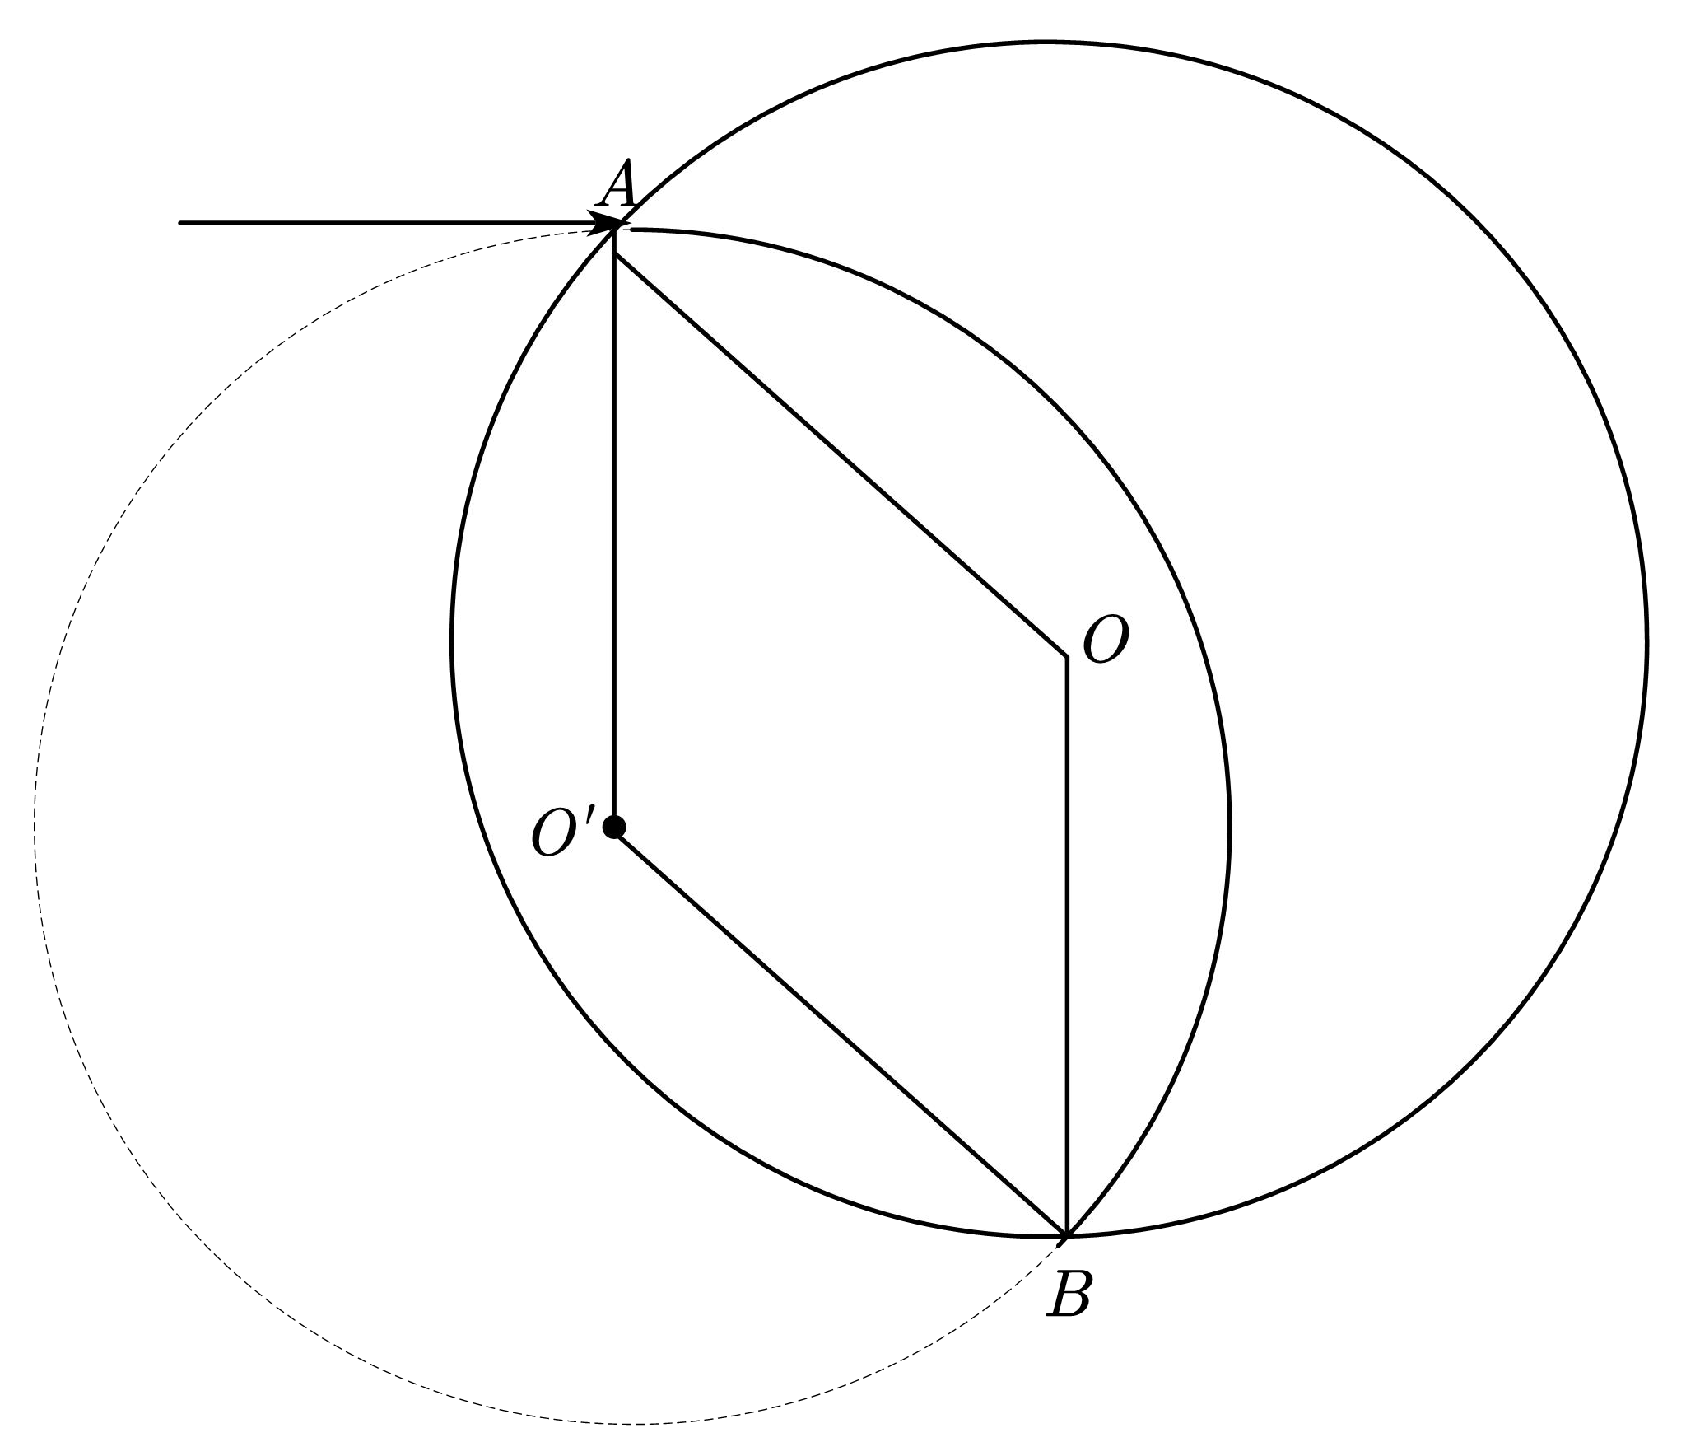
\includegraphics[width=0.7\linewidth]{../LatePic/CJJZM}
		\caption*{}
		\label{fig:cjjzm}
	\end{figure}
	如图, $AOBO'$ 是菱形, 因为 $AO'$ 是竖直的,所以 $OB$ 也是竖直的,证毕.
	\nonumbersubsection{(2)}
	\begin{figure}[H]
		\centering
		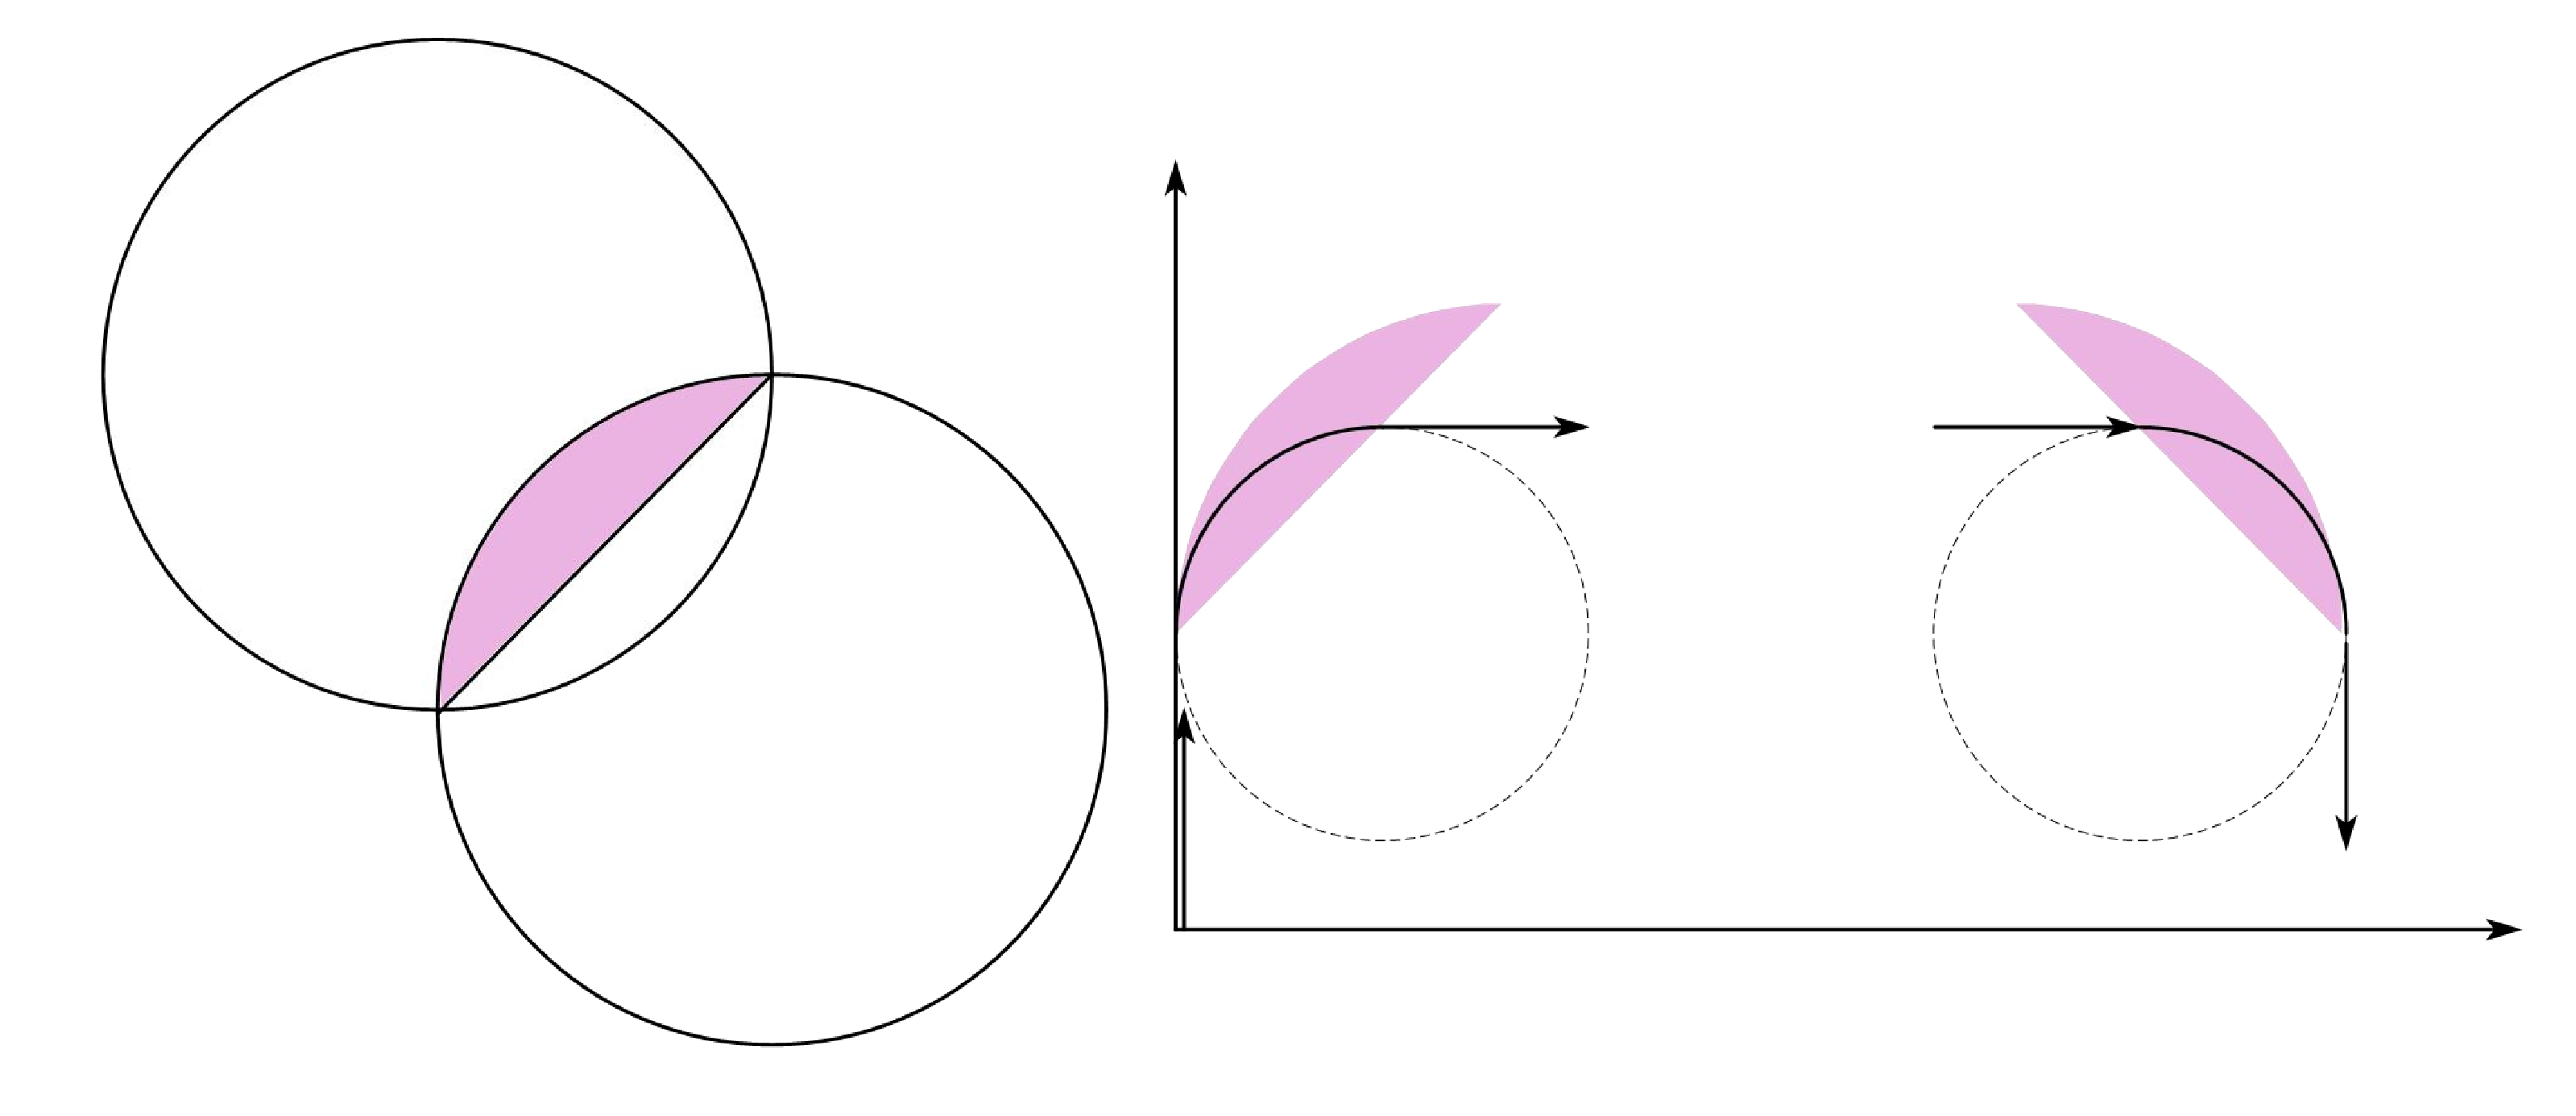
\includegraphics[width=1\linewidth]{../LatePic/CCSJ}
		\caption*{}
		\label{fig:ccsj}
	\end{figure}
	运用上一题的结论, 设计磁场的边界半径为
	\begin{equation}
		R_B=\dfrac{mv_0}{qB}
	\end{equation}
	为了让不同运动半径的粒子都能水平出射, 以一条倾斜 $\dfrac{\pi}{4}$ 的斜线作为磁场的另一个边界,因为 $OA$ 足够远, 所以两片磁场不会相交, 因为粒子带正电, 所以磁场方向应该是垂直纸面向外.
	\nonumbersubsection{(3)}
	\begin{figure}[H]
		\centering
		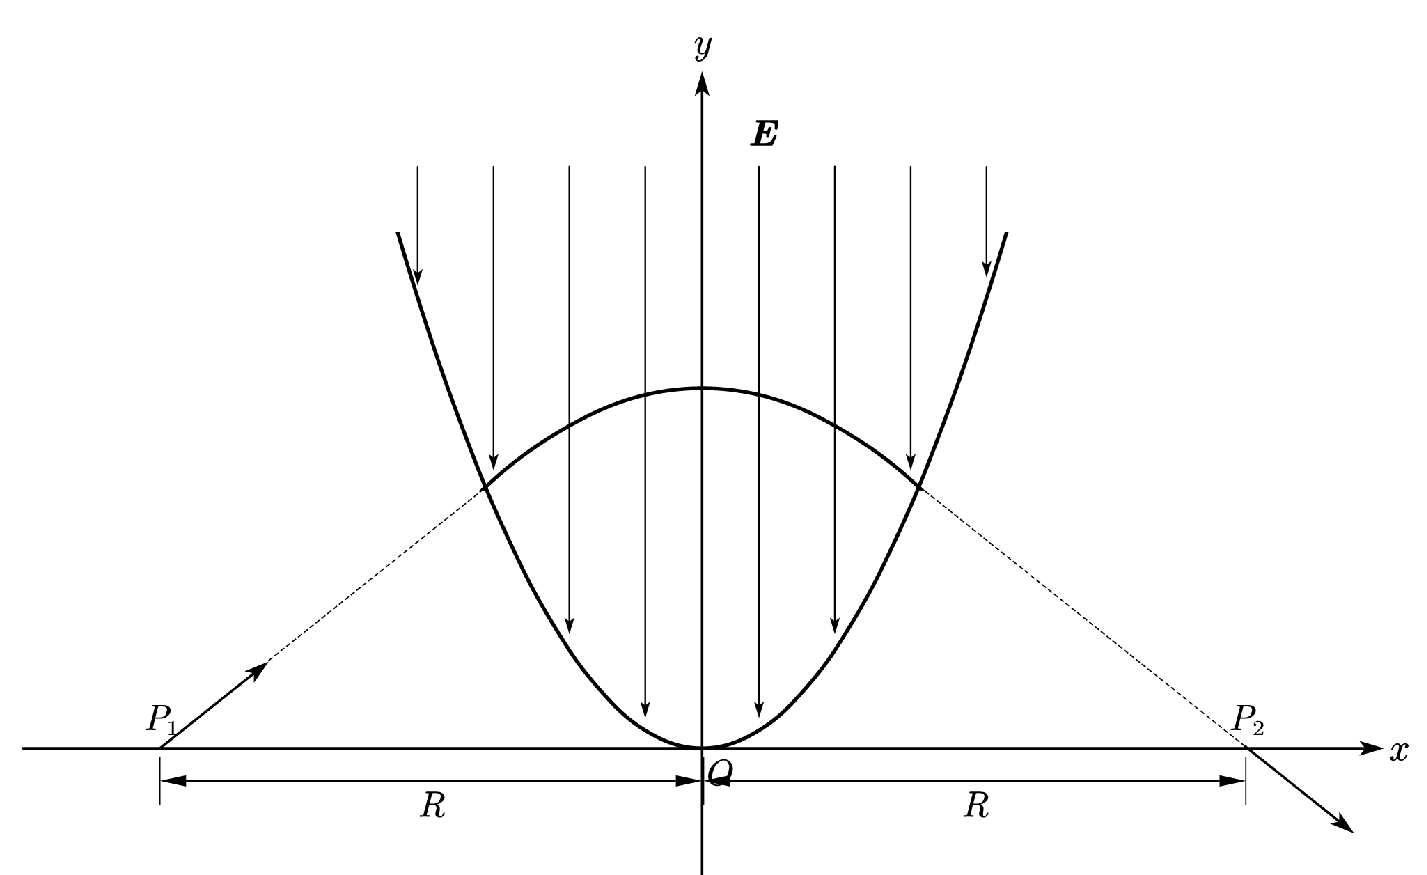
\includegraphics[width=1\linewidth]{../LatePic/DCSJ}
		\caption*{}
		\label{fig:dcsj}
	\end{figure}
	设计如图匀强电场, 在右侧边界上任取一点 $(x,y)$, 考究粒子在场内的运动, 由运动学
	\begin{equation}
		x=v_0\cos\phi\Delta t
	\end{equation}
	\begin{equation}
		v_0\sin\phi=a\Delta t
	\end{equation}
	牛顿第二定律给出加速度的大小
	\begin{equation}
		ma=qE
	\end{equation}
	根据几何关系又有
	\begin{equation}
		\sin\phi=\dfrac{y}{\sqrt{y^2+(R-x)^2}}\qquad\cos\phi=\dfrac{R-x}{\sqrt{y^2+(R-x)^2}}
	\end{equation}
	得到:
	\begin{equation}
		v_{0}^{2}y\left( R-x \right) =\frac{qE}{m}\left[ y^2+(R-x)^2 \right] \qquad x\geqslant 0
	\end{equation}
	由对称性, 左边界为
	\begin{equation}
		v_{0}^{2}y\left( R+x \right) =\frac{qE}{m}\left[ y^2+(R+x)^2 \right] \qquad x\leqslant 0
	\end{equation}
	合起来就是
	$$
	v_{0}^{2}y\left( R\pm x \right) =\frac{qE}{m}\left[ y^2+(R\pm x)^2 \right]
	$$
	\nonumbersubsection{*(4)}
	注意, 本大题的解法\textbf{不唯一}. 其他解法只要能准确描述场的边界的并且证明结论即可.
	\section*{第二题}
	\nonumbersubsection{(1)}
	\nonumbersubsubsection{(i)}
	考究无穷大平板, 在其上任取一点为参考点, 则平板上任意一点的速度可视作绕参考点的转动和平动的矢量和. 若参考点速度为零, 则它就是瞬心, 若否, 则由于平板无限大, 所以任意的平动速度矢量 $\boldsymbol{v}$, 都可以在平板上距参考点 $r=v/\omega\ (\omega\text{是绕参考点转动的角速度})$ 的圆周上找到一点, 该点速率为 $v$, 速度方向与 $\boldsymbol{v}$ 相反(通过找到相对参考点的角度), 转动的速度和平动的速度的矢量和就是 $\boldsymbol{0}$, 这个点就是顺心.
	
	对于给定的刚体, 视作从无穷大平板上截取的, 它的速度顺心就是这个.
	
	\nonumbersubsubsection{(ii)}
	\begin{figure}[H]
		\centering
		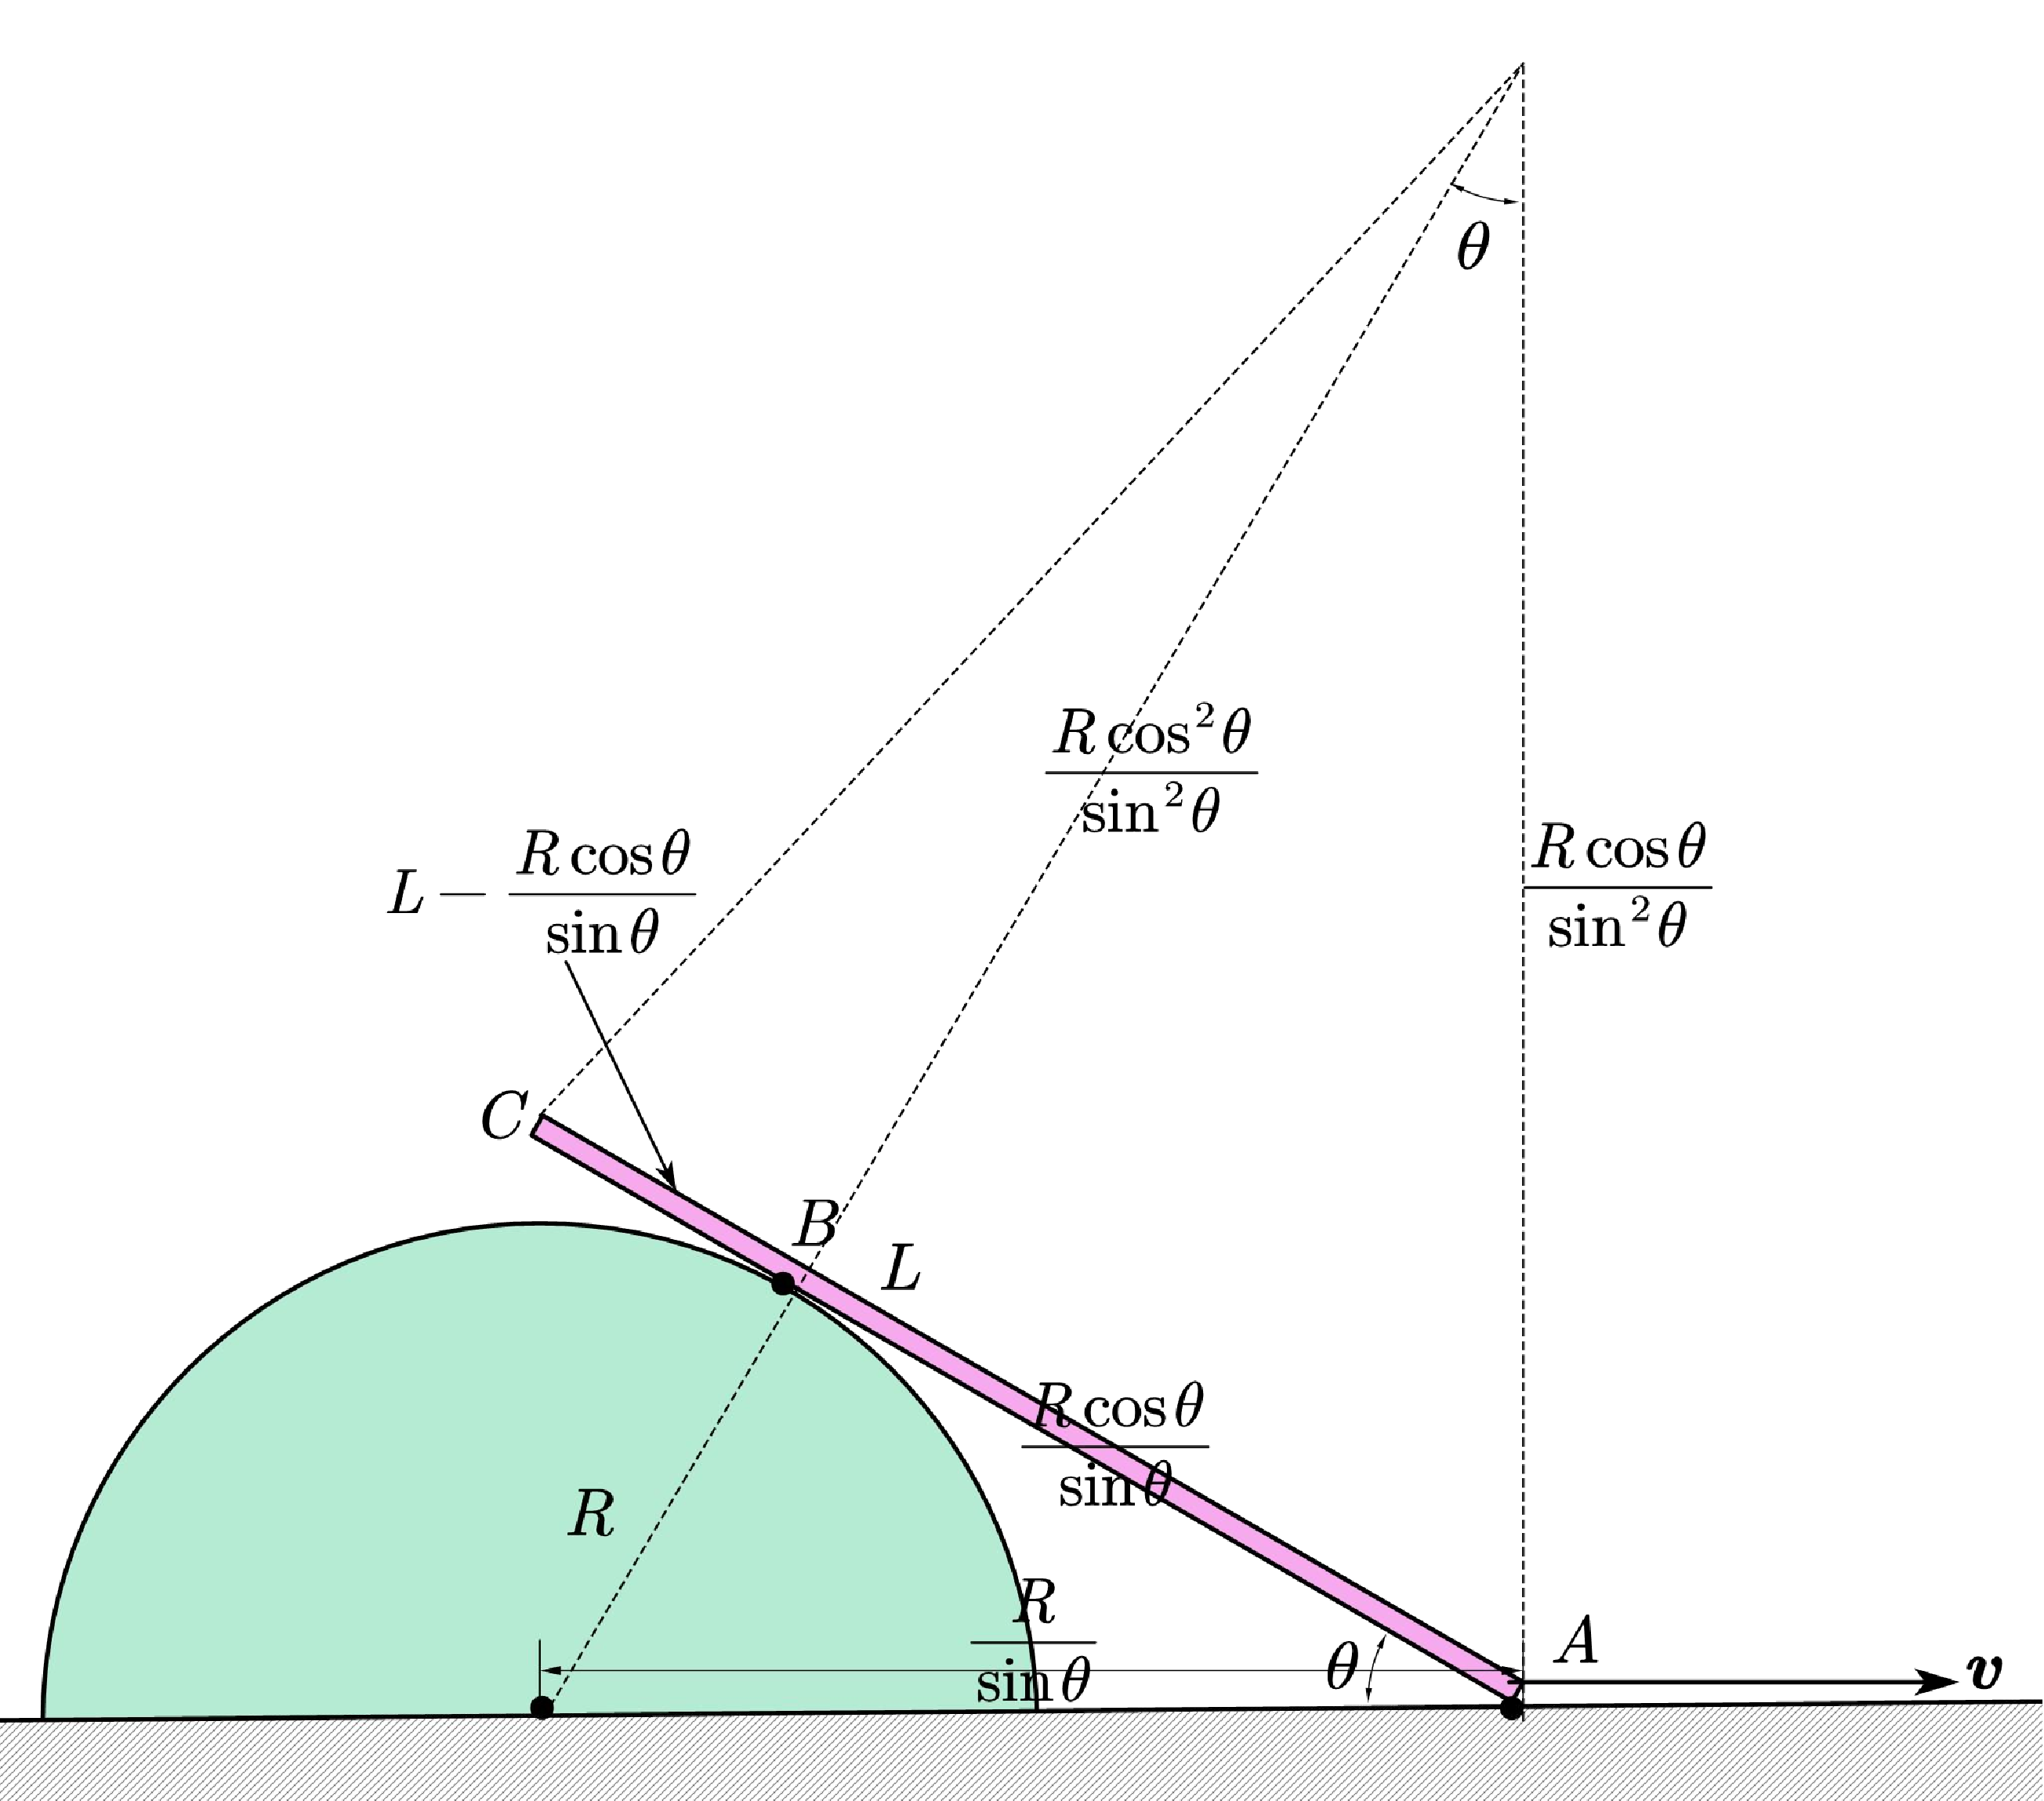
\includegraphics[width=0.7\linewidth]{../LatePic/JDZXjie}
		\caption*{}
		\label{fig:jdzxjie}
	\end{figure}
	如图所示, 过 $A$ 点和 $B$ 点作各自速度的垂线, 两线交点即速度顺心, 根据几何关系容易求出 $C$ 点到顺心的距离 $r $ 为:
	\begin{equation}
		r_C=\sqrt{\left( L-R\cot\theta\right)^2 + R^2\cot^4\theta }
	\end{equation}
	
	
	根据顺心的性质:
	\begin{equation}
		\omega=\dfrac{v}{r_A}=\dfrac{v\sin^2\theta}{R\cos\theta}
	\end{equation}
	
	所以最终:
	$$
	v_C=\omega r_C=\dfrac{v}{r_A}=\dfrac{v\sin^2\theta}{R\cos\theta}\sqrt{\left( L-R\cot\theta\right)^2 + R^2\cot^4\theta }
	$$
	\nonumbersubsection{(2)}
	\begin{figure}[H]
		\centering
		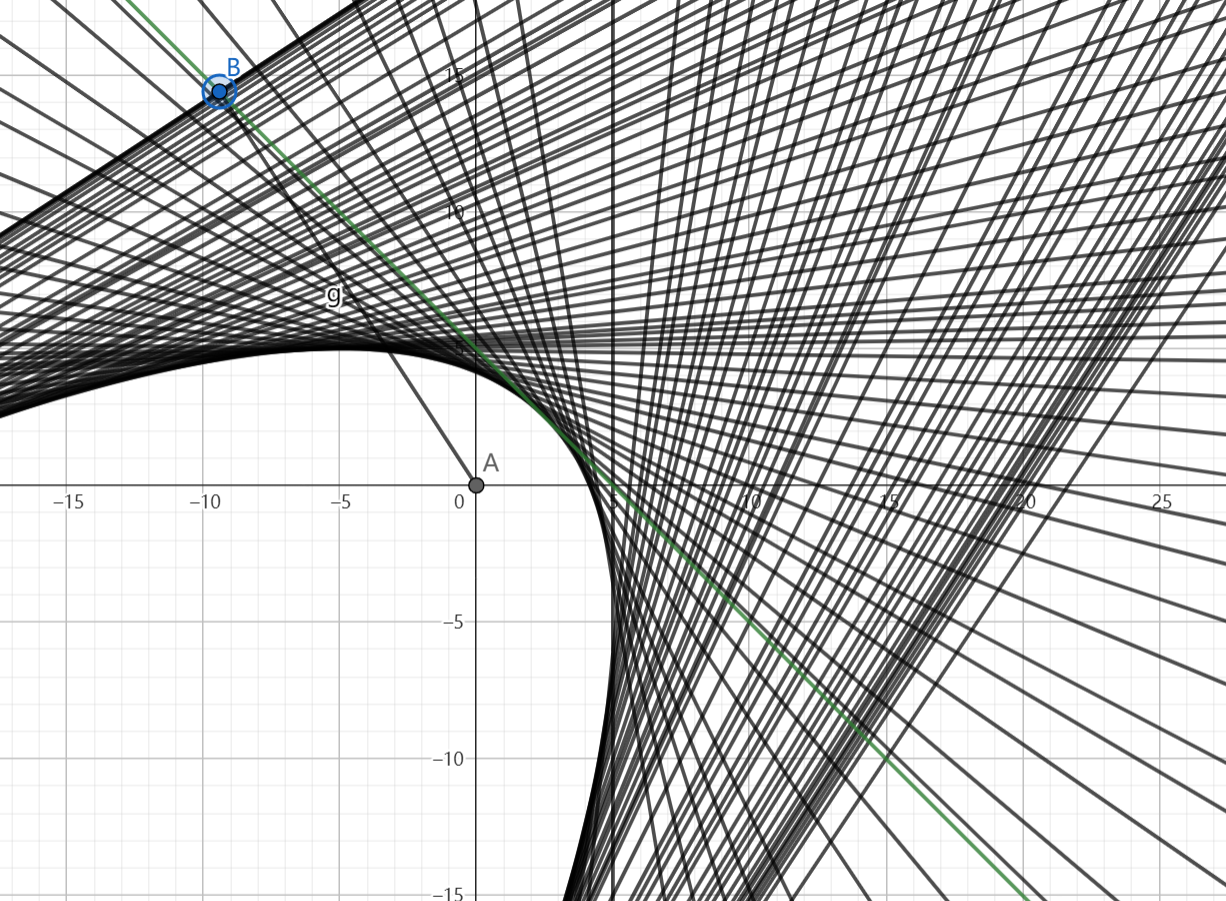
\includegraphics[width=0.8\linewidth]{../LatePic/BLM}
		\caption*{}
		\label{fig:blm}
	\end{figure}
	\begin{figure}[H]
		\centering
		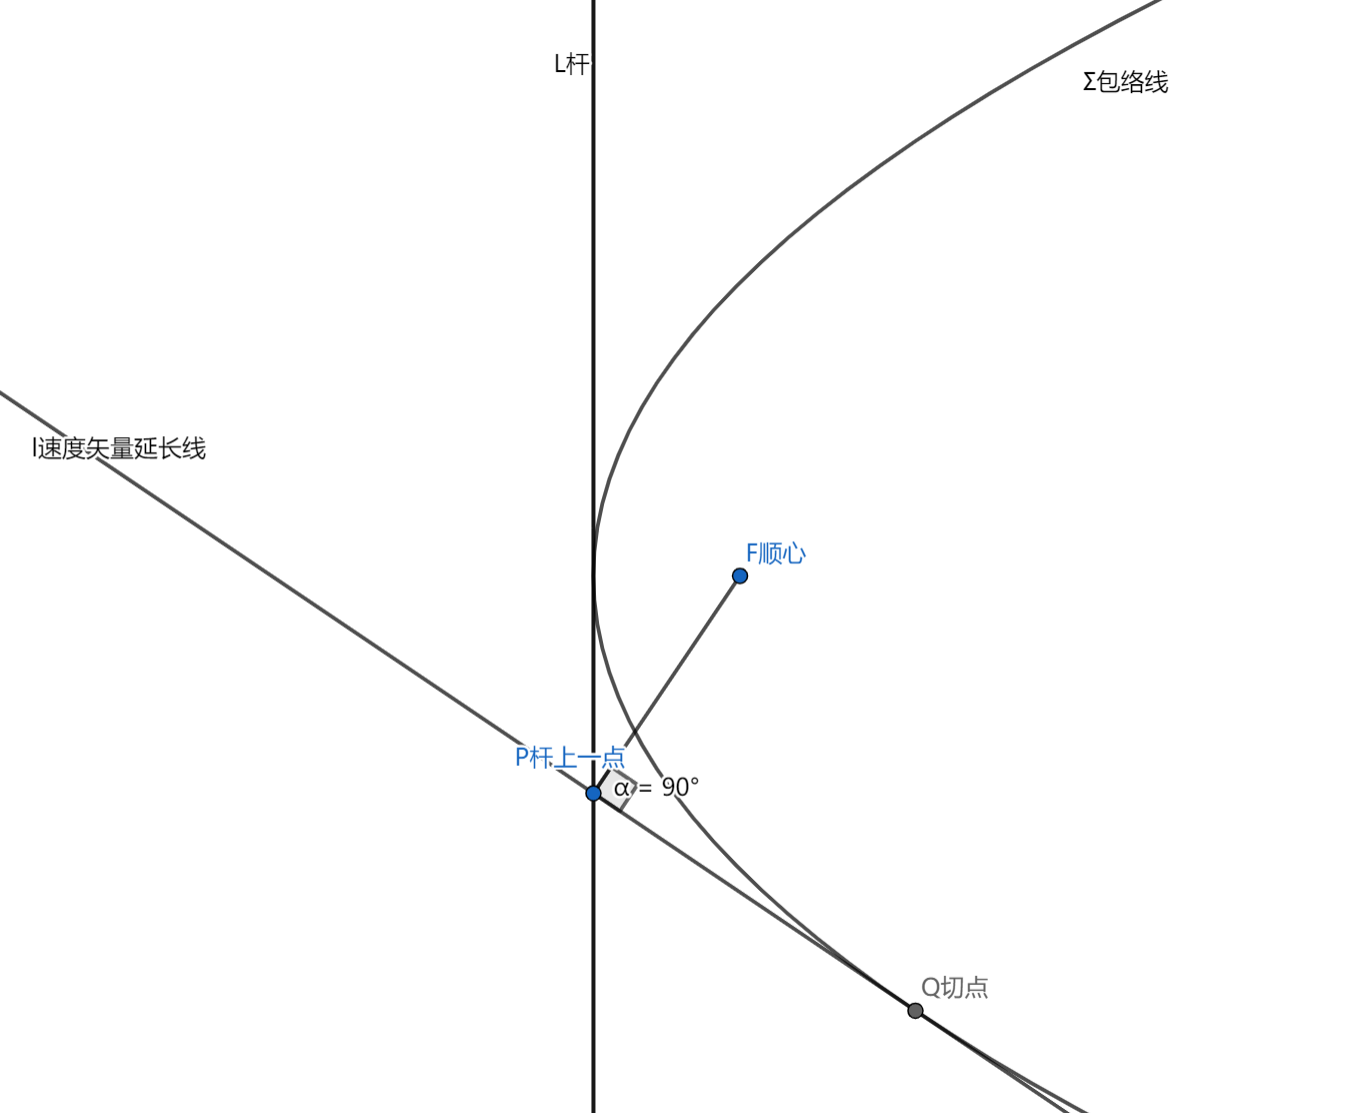
\includegraphics[width=0.8\linewidth]{../LatePic/SYT}
		\caption*{}
		\label{fig:syt}
	\end{figure}
	形状: 抛物线
	
	证明: 根据瞬心的性质, 速度矢量的延长线与瞬心和该点的连线垂直,考究解析几何.
	显然, 杆将平面分为了两片区域, 没有瞬心的一侧显然能被速度矢量的延长线填充, 考虑瞬心所在那一侧. 如图所示 $P$ 点是在杆上任取的一点, 顺心是 $F$ 点,速度矢量延长线设为 $l$, 其垂直于 $PF$, 只需证明 $l$ 与以 $F$ 点为焦点的抛物线相切即可.
	
	设 $\Sigma: y^2=2px, F(\dfrac{p}{2},0), P(0,y_0)$, 那么 $l: y=\dfrac{p}{2y_0}x+y_0$, 与 $\Sigma$ 联立得到:
	\begin{equation}
		x^2-\dfrac{4y_0^2}{p}x+\dfrac{4y_0^4}{p^2}=0
	\end{equation}
	显然 $\Delta=0$, 唯一的解为 $x=\dfrac{2y_0}{p}$. 也就是说, 任意速度矢量的延长线与以速度顺心为焦点的抛物线只有一个交点, 所以速度矢量的延长线的包络就是这个抛物线.
	
	采用包络线方程组的方法直接解出包络线方程也是可以的. 
	
	定理: 关于参数 $\theta$ 的曲线簇 $F\left( x,y,\theta \right) =0$ 的包络满足方程组:
	\begin{align}
		\left\{ \begin{array}{c}
			F\left( x,y,\theta \right) =0\\
			\\
			\dfrac{\partial F}{\partial \theta}=0\\
		\end{array} \right. 
	\end{align}
	其中 $\dfrac{\partial}{\partial\theta}$ 表示对 $F$ 求 $\theta$ 的偏导数, 也就是将 $\theta$ 视为主变量其他变量视为参数求一次导数. 代入 $F=l,\theta=y_0$ 并消除 $y_0$, 得到的方程就是包络抛物线的方程.
	\section*{第三题}
	\nonumbersubsection{(1)}
	设虚位移为 $\delta x$
	\begin{equation}
		T\delta x=\delta x\lambda gR
	\end{equation}
	解得
	$$
	T=\lambda gR
	$$
	\nonumbersubsection{(2)}
	受力分析和虚功原理得到
	\begin{equation}
		(T_2-T_1)\delta x=\lambda \delta xgh
	\end{equation}
	\begin{equation}
		T_1\sin\alpha=T_2\sin\beta
	\end{equation}
	\begin{equation}
		T_1\cos \alpha +T_2\cos \beta =\lambda Lg
	\end{equation}
	解得
	$$
	\beta=\arcsin\dfrac{L\sin\alpha}{\sqrt{\left( L+h\cos\alpha\right)^2+\left( h\sin\alpha\right)^2  }}-\arctan\dfrac{h\sin\alpha}{L+h\cos\alpha}
	$$
	\nonumbersubsection{(3)}
	以 $A$ 为原点, $AO$ 为 $z$ 轴, 垂直 $BC$ 的方向为 $x$ 轴, 建立右手坐标系
	\begin{figure}[H]
		\centering
		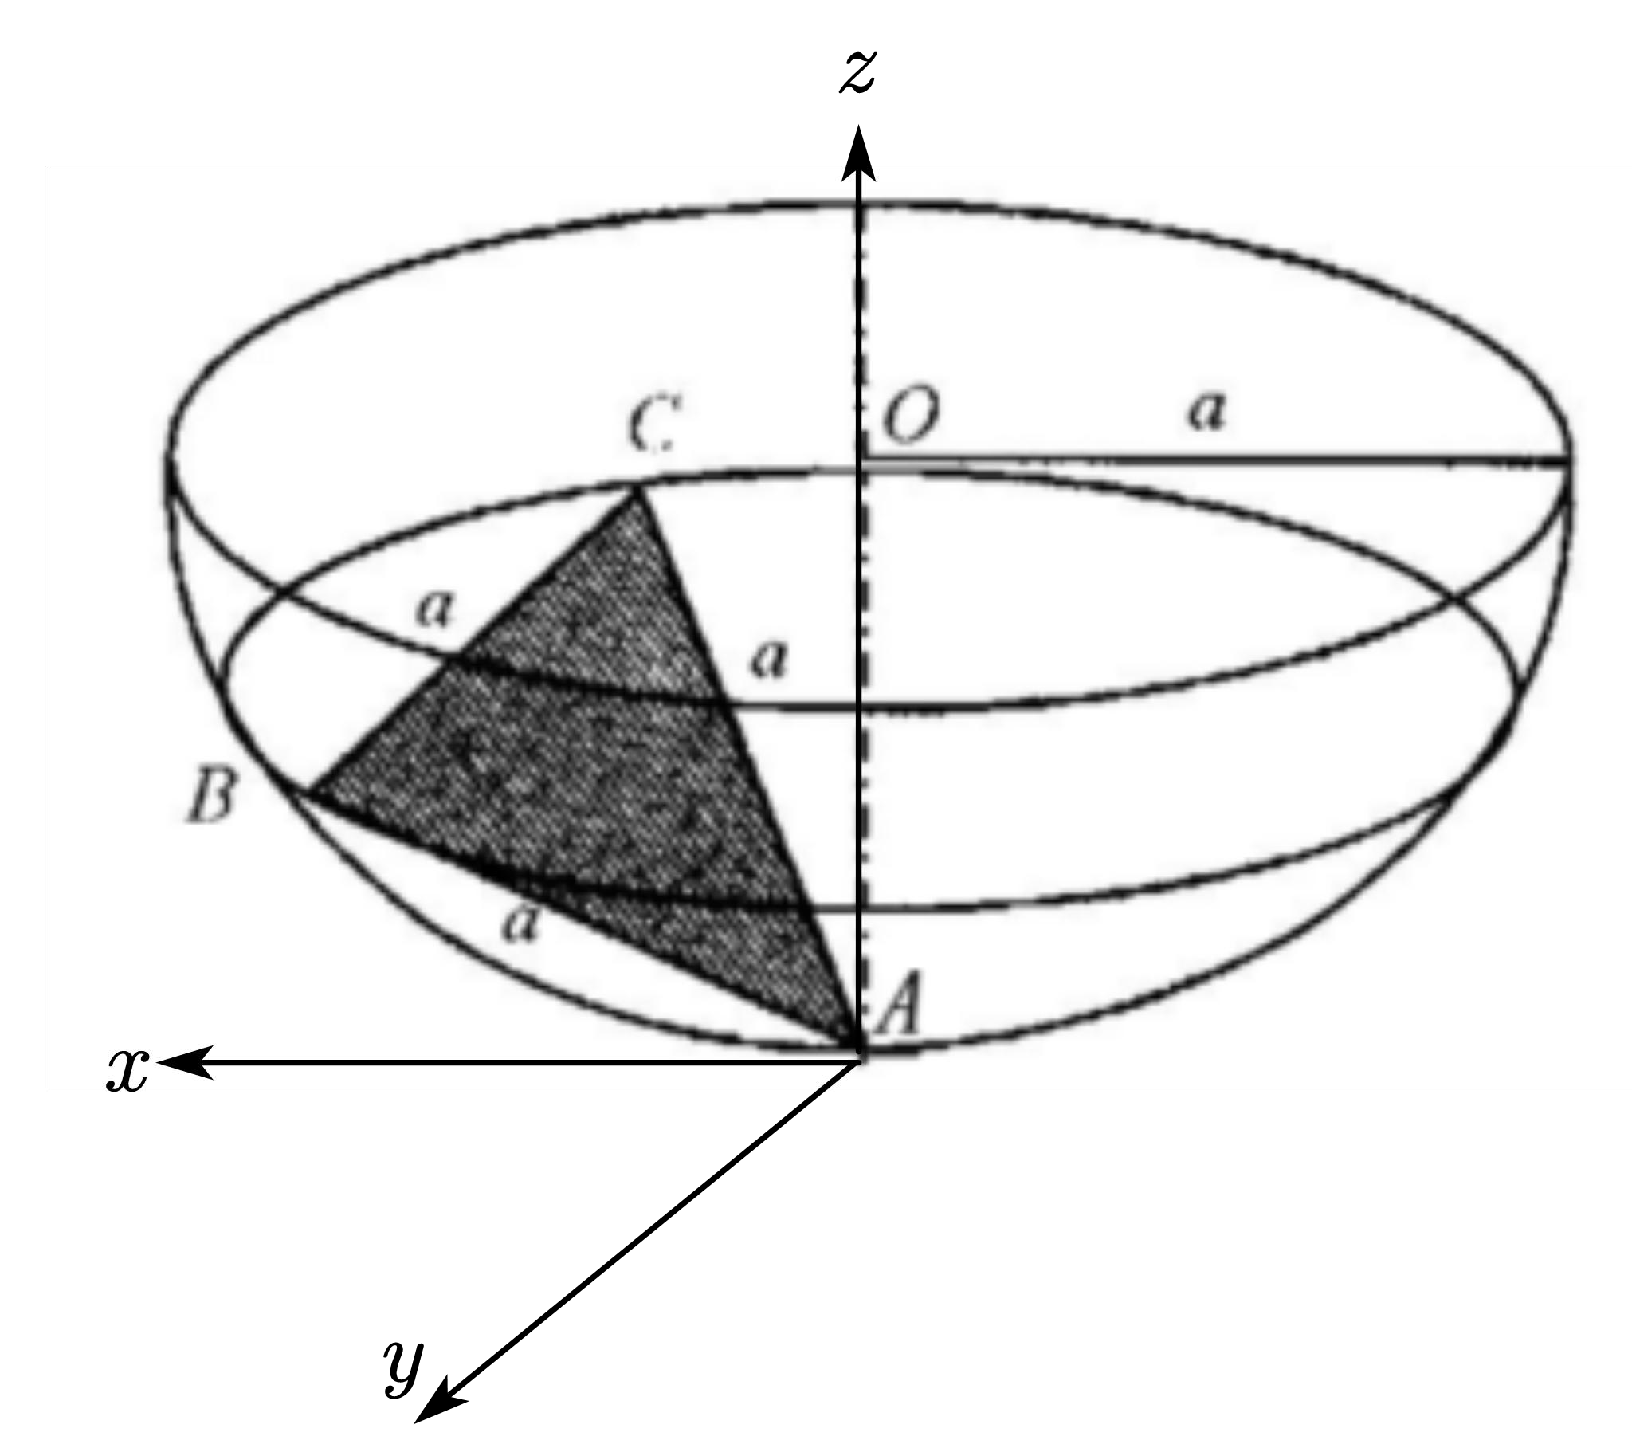
\includegraphics[width=0.7\linewidth]{../LatePic/WNYQ}
		\caption*{}
		\label{fig:wnyq}
	\end{figure}
	容易得到 $B\left(\dfrac{1}{\sqrt{2}}a,\dfrac{1}{2}a,\dfrac{1}{2}a\right),C\left(-\dfrac{1}{\sqrt{2}}a,\dfrac{1}{2}a,\dfrac{1}{2}a\right),\overrightarrow{BO}=\left( -\sqrt{2},-1,1 \right),\overrightarrow{CO}=\left( -\sqrt{2},1,1 \right)$. 显然 $N_B=N_C$, 各自的方向都是指向圆心 $O$, 那么
	\begin{equation}
		\boldsymbol{N}_B=N_B\dfrac{\overrightarrow{BO}}{|\overrightarrow{BO}|}
	\end{equation}
	\begin{equation}
		\boldsymbol{N}_C=N_C\dfrac{\overrightarrow{CO}}{|\overrightarrow{CO}|}
	\end{equation}
	注意到 $\boldsymbol{e}=\left( 1,0,-\sqrt{2} \right) $ 是平面 $ABC$ 的一个法向量, 设 $B$ 点绕 $AC$ 有一个极小的转动, 则虚位移为
	\begin{equation}
		\delta \boldsymbol{x}=\delta x\dfrac{\boldsymbol{e}}{|\boldsymbol{e}|}
	\end{equation}
	设 $G$ 是板的重心, 根据三角形的重心公式得
	\begin{equation}
		G\left( \dfrac{x_A+x_B+x_C}{3},\dfrac{y_A+y_B+y_C}{3},\dfrac{z_A+z_B+z_C}{3}\right) 
	\end{equation}
	则 $G$ 的虚位移为
	\begin{equation}
		\delta\boldsymbol{x}_G=\dfrac{1}{3}\delta\boldsymbol{x}
	\end{equation}
	根据虚功原理
	\begin{equation}
		\boldsymbol{N}_B\cdot\delta \boldsymbol{x}+\boldsymbol{G}\cdot\delta\boldsymbol{x}_G=0
	\end{equation}
	其中 $\boldsymbol{G}=\left(0,0,-mg \right) $ 是三角形板受到的重力.
	解得
	$$
	N_B=\dfrac{1}{3}mg
	$$
	据此
	$$
	\boldsymbol{N}_B=\left( -\dfrac{\sqrt{2}}{2},-\dfrac{1}{2},\dfrac{1}{2}\right) \dfrac{1}{3}mg
	$$
	$$
	\boldsymbol{N}_C=\left( -\dfrac{\sqrt{2}}{2},\dfrac{1}{2},\dfrac{1}{2}\right) \dfrac{1}{3}mg
	$$ 
	根据受力矢量和为零可以解出 $A$ 点受力
	$$
	\boldsymbol{N}_A=\left( \dfrac{1}{\sqrt{3}},0,\dfrac{\sqrt{2}}{\sqrt{3}}\right) \dfrac{\sqrt{2}}{\sqrt{3}}mg
	$$
	\section*{第四题}
	\nonumbersubsection{(1)}
	\nonumbersubsubsection{(i)}
	考虑体积为 $V$, 底面积为 $S$ 的正方形刚性容器内装有物质的量为 $n$ 的理想气体在较短的一段时间 $\Delta t$ 内的运动, 对容器沿 $x$ 方向一面受力分析:
	\begin{equation}
		p=\dfrac{F}{S}=\dfrac{1}{S}\dfrac{\Delta P}{\Delta t}
	\end{equation}
	其中 $\Delta P$ 为力 $F$ 在时间 $\Delta t$ 内引起的粒子群的动量变化
	\begin{equation}
		\Delta P = \dfrac{1}{2}v_x\Delta tS\dfrac{nN_\mathrm{A}}{V}2mv_x=\dfrac{nN_\mathrm{A}}{V}mv_x^2S\Delta t
	\end{equation}
	其中, 系数 $\dfrac{1}{2}$ 表示 $x$ 方向上仅有一半数目的粒子速度为正, $\dfrac{1}{2}v_x\Delta tS\dfrac{nN_\mathrm{A}}{V}$ 表示时间 $\Delta t$ 内会和容器面相撞的粒子数.
	同时认为
	\begin{equation}
		\dfrac{1}{2}mv_x^2=\dfrac{1}{3}\dfrac{1}{2}mv^2=\dfrac{1}{2}k_{\mathrm{B}}T
	\end{equation}
	整理得到
	$$
	pV=nN_\mathrm{A}k_\mathrm{B}T
	$$
	此即理想气体状态方程, 不难得到 $R=N_\mathrm{A}k_\mathrm{B}$.
	\nonumbersubsubsection{(ii)}
	取一个微小过程, 考虑容器被压缩了极小的体积 $\Delta V$, 方程满足
	\begin{equation}
		\Delta \left(pV^\gamma \right) =0
	\end{equation}
	根据导数的运算规则
	\begin{equation}
		\Delta pV^\gamma+\gamma pV^{\gamma-1}\Delta V=0
	\end{equation}
	进一步
	\begin{equation}
		\Delta pV+\gamma p\Delta V=0
		\label{27}
	\end{equation}
	理想气体地内能仅与温度相关
	\begin{equation}
		U=N\dfrac{1}{2}mv^2=nN_\mathrm{A}\dfrac{3}{2}k_\mathrm{B}T
	\end{equation}
	根据热力学第一定律
	\begin{equation}
		\Delta U=Q+W
	\end{equation}
	其中, $Q=0$, $W=-p\Delta V$, 此处为不失一般性设 $\Delta V<0$, 因此
	\begin{equation}
		nN_\mathrm{A}\dfrac{3}{2}k_\mathrm{B}\Delta T=-p\Delta V
	\end{equation}
	与此同时考虑理想气体状态方程
	\begin{equation}
		\Delta\left(pV \right)=\Delta pV+p\Delta V =nN_\mathrm{A}k_\mathrm{B}\Delta T
	\end{equation}
	联立得
	\begin{equation}
		\Delta pV+\dfrac{5}{3}p\Delta V=0
	\end{equation}
	与(\ref{27})对比得到 $\gamma =\dfrac{5}{3}$.
	\nonumbersubsection{(2)}
	方法一:直接联立绝热曲线和等温曲线
	\begin{equation}
		pV^{\tfrac{5}{3}}=pV
	\end{equation}
	这个方程有且仅有一个解.
	
	方法二:构造一个热力学循环导出矛盾
	\begin{figure}[H]
		\centering
		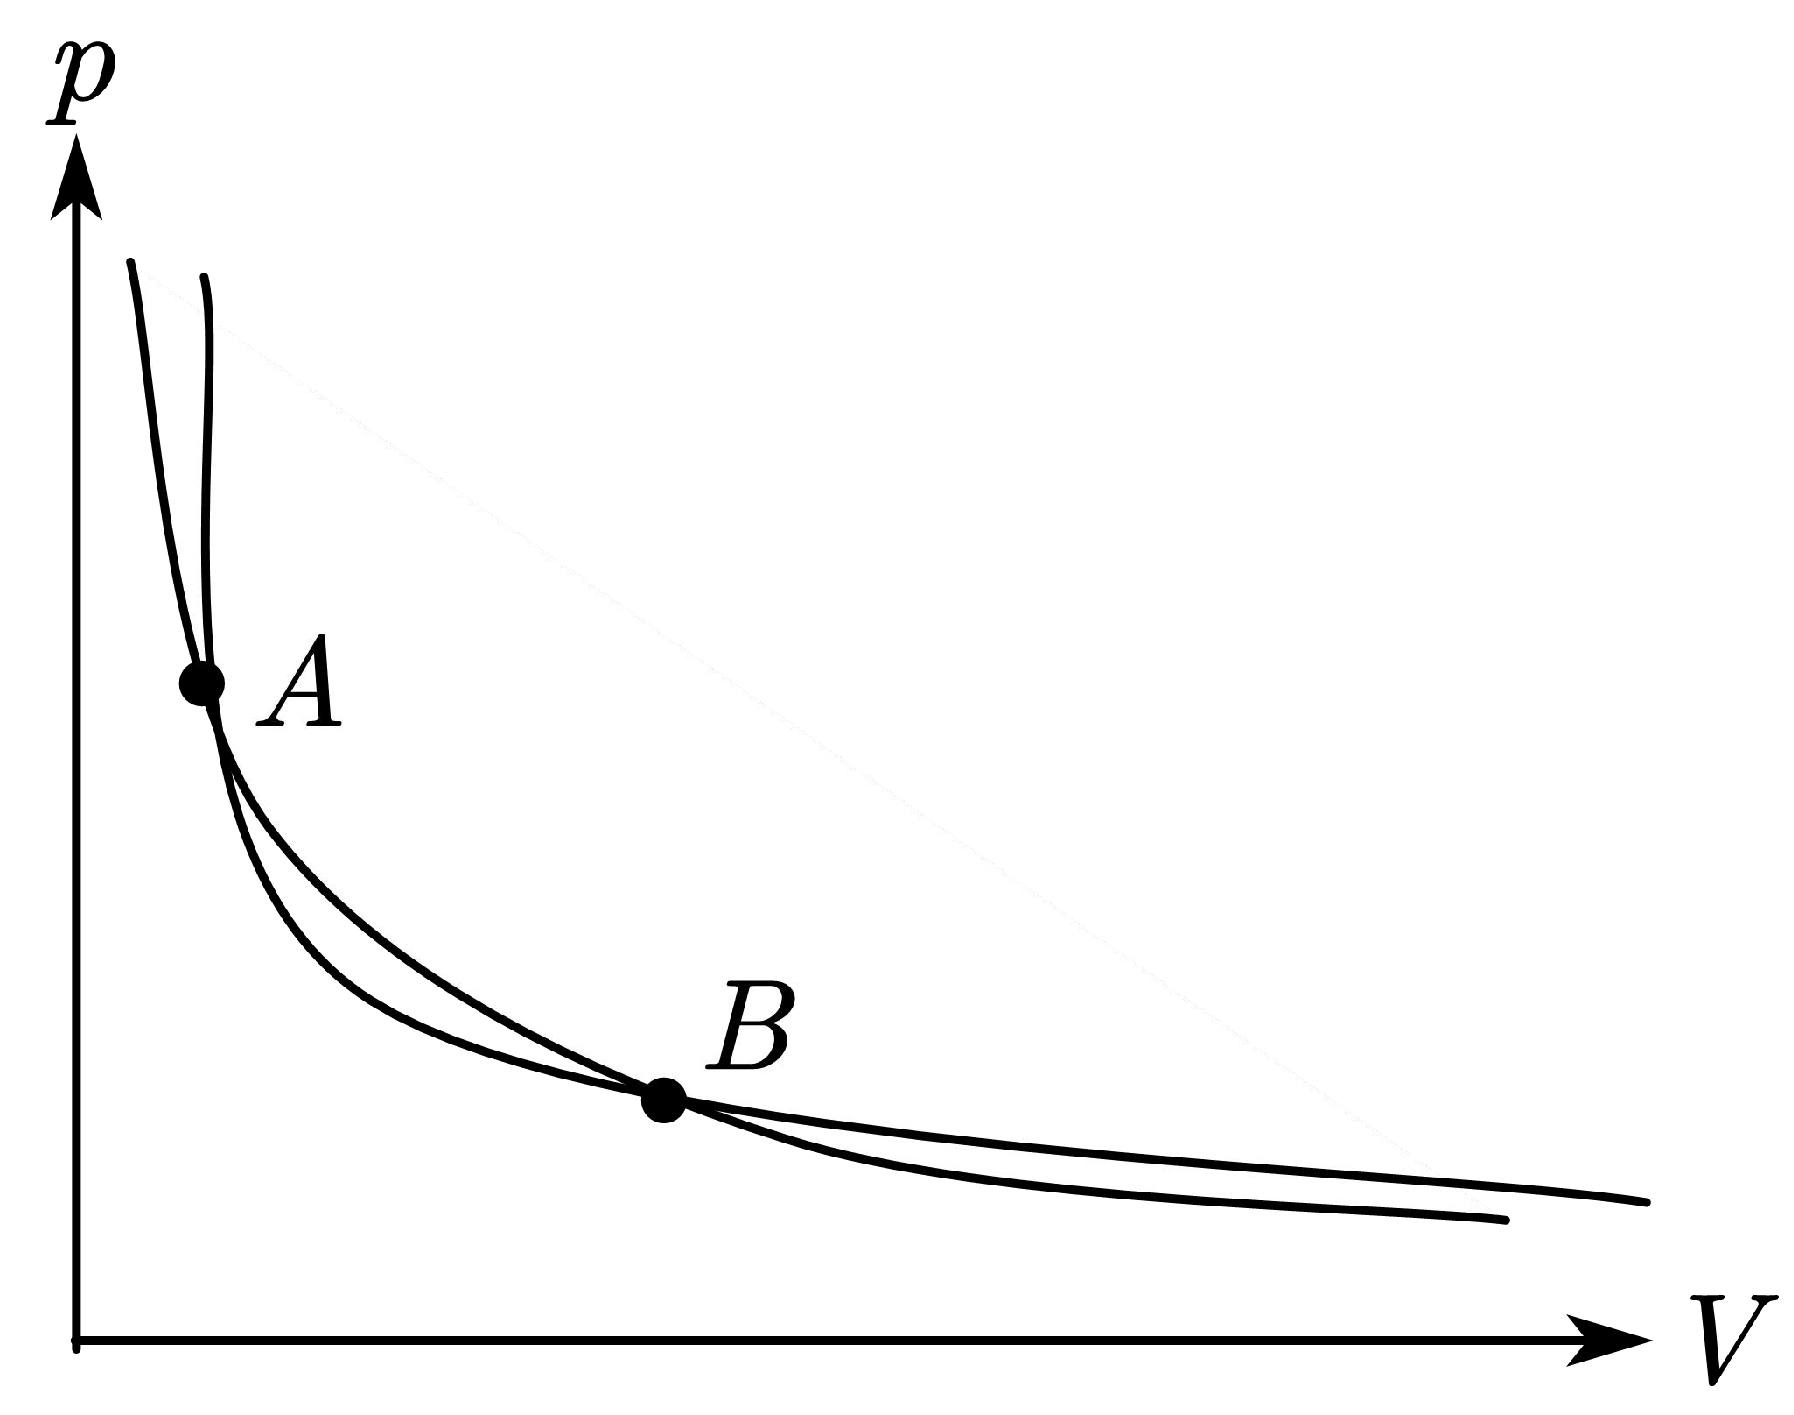
\includegraphics[width=0.7\linewidth]{../LatePic/P_V}
		\caption*{}
		\label{fig:pv}
	\end{figure}
	假设两曲线有两个或以上的交点, 取相邻的两个交点命名为 $A$、$B$, 设气体从 $A$ 绝热膨胀到 $B$, 则气体对外做功降温, 内能减少, 在让气体等温压缩回到 $A$, 过程中气体内能不变, 所以
	\begin{equation}
		U_A>U_B=U_A
	\end{equation}
	导出了矛盾.
	\section{第五题}
	\nonumbersubsection{(1)}
	\nonumbersubsubsection{(i)}
	如图所示, $A$ 点和 $A'$ 点是中心对称的, 假设发生反射的点偏移了 $\delta L$ 的距离, 则新的光路的光程为
	\begin{figure}[H]
		\centering
		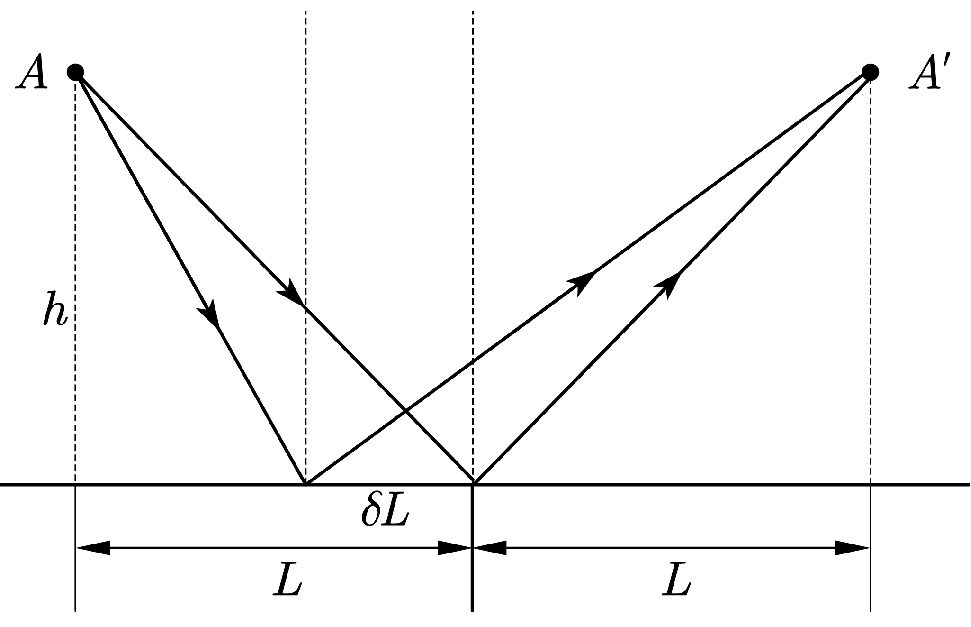
\includegraphics[width=0.7\linewidth]{../LatePic/JSDL}
		\caption*{}
		\label{fig:jsdl}
	\end{figure}
	\begin{equation}
		S(\delta L)=\sqrt{h^2+\left(L-\delta L \right)^2 }+\sqrt{h^2+\left(L+\delta L \right)^2 }
	\end{equation}
	
	根据凹函数的性质:
	\begin{align}
		S(\delta L)&=\sqrt{h^2+\left(L-\delta L \right)^2 }+\sqrt{h^2+\left(L+\delta L \right)^2 }\nonumber
		\\\nonumber
		\\
		&\geqslant 2\sqrt{h^2+\left( \dfrac{\left( L-\delta L\right)+\left( L+\delta L\right)  }{2}\right)^ 2}\nonumber
		\\\nonumber
		\\
		&=2\sqrt{h^2+L^2}=S(0)\nonumber
	\end{align}
	
	也就是说任何不在对称轴处发生的反射都会使得光程变大, 违背了费马原理, 所以反射一定会发生在对称轴上.
	
	\begin{figure}[H]
		\centering
		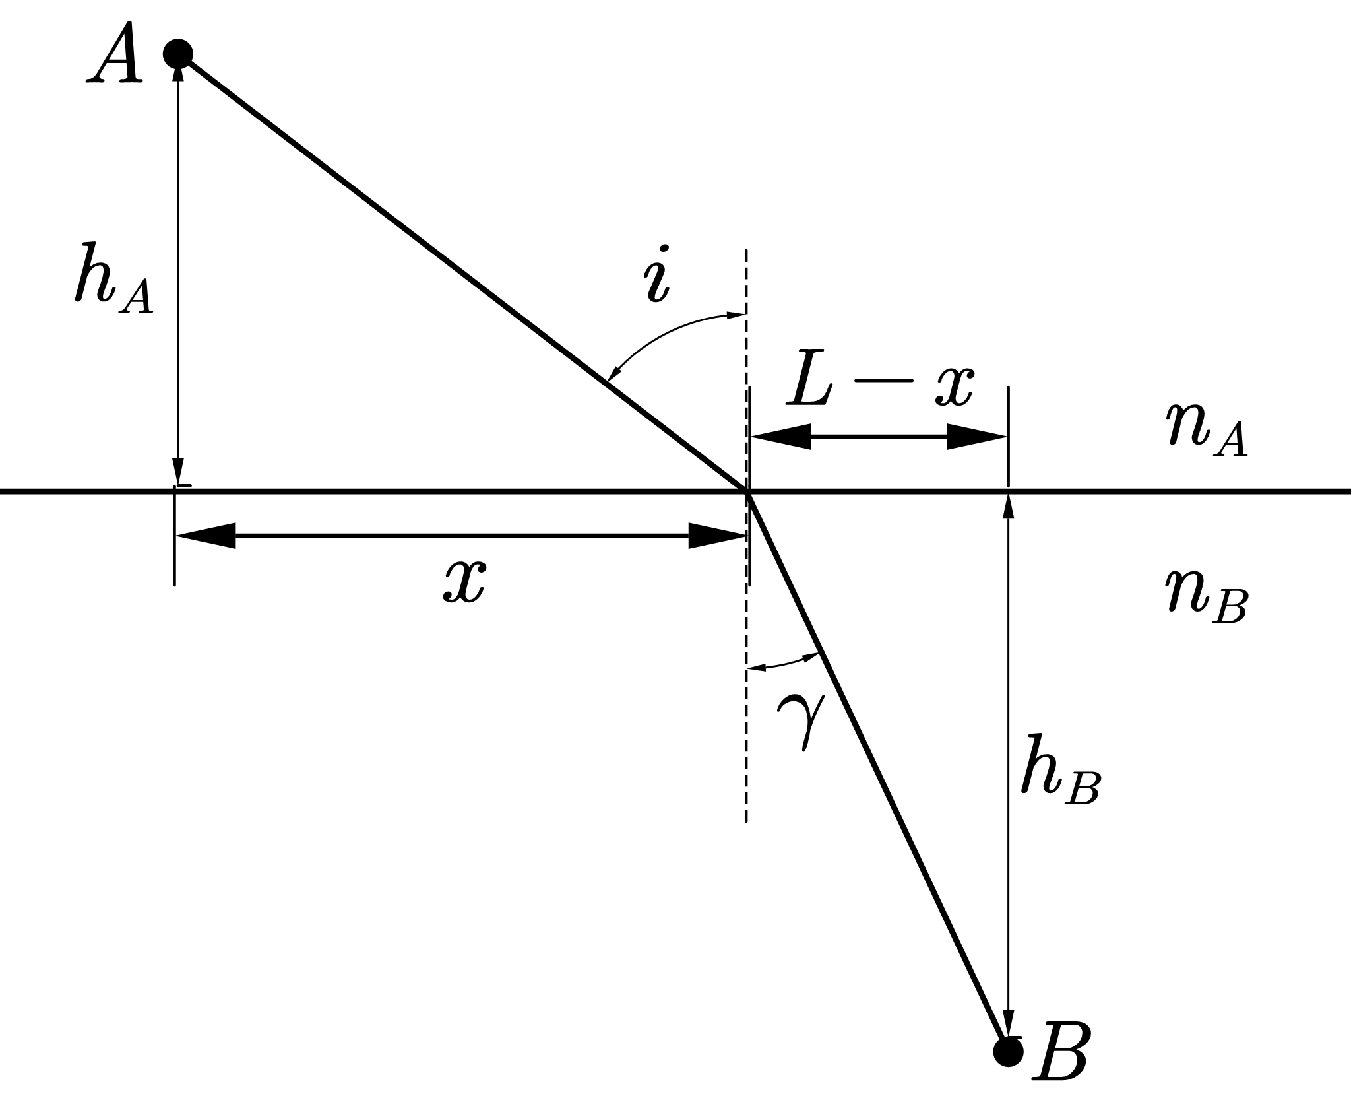
\includegraphics[width=0.7\linewidth]{../LatePic/JSSSDL}
		\caption*{}
		\label{fig:jsssdl}
	\end{figure}
	
	折射定律也可以用同样的方法证明:
	\begin{equation}
		S(x)=n_A\sqrt{h_A^2+x^2}+n_B\sqrt{h_B^2+(L-x)^2}
	\end{equation}
	对 $x$ 求一次导数:
	\begin{equation}
		S'(x)=\dfrac{n_Ax}{\sqrt{h_A^2+x^2}}-\dfrac{n_B\left( L-x\right) }{\sqrt{h_B^2+\left(L-x \right)^2 }}
	\end{equation}
	令 $S'(x)=0$ 并代入 $\sin i=\dfrac{x}{\sqrt{h_A^2+x^2}}, \sin\gamma=\dfrac{\left( L-x\right) }{\sqrt{h_B^2+\left(L-x \right)^2 }}$, 解得:
	$$
	n_A\sin i=n_B\sin \gamma
	$$
	\nonumbersubsubsection{(ii)}
	\textbf{根据折射定律}, 入水点满足
	\begin{equation}
		\dfrac{x}{\sqrt{h_A^2+x^2}}=\dfrac{n\left( L-x\right) }{\sqrt{h_B^2+\left(L-x \right)^2 }}
	\end{equation}
	其中 $x$ 是入水点沿水陆交界线离救生员的距离. 
	\nonumbersubsubsection{(iii)}
	\begin{figure}[H]
		\centering
		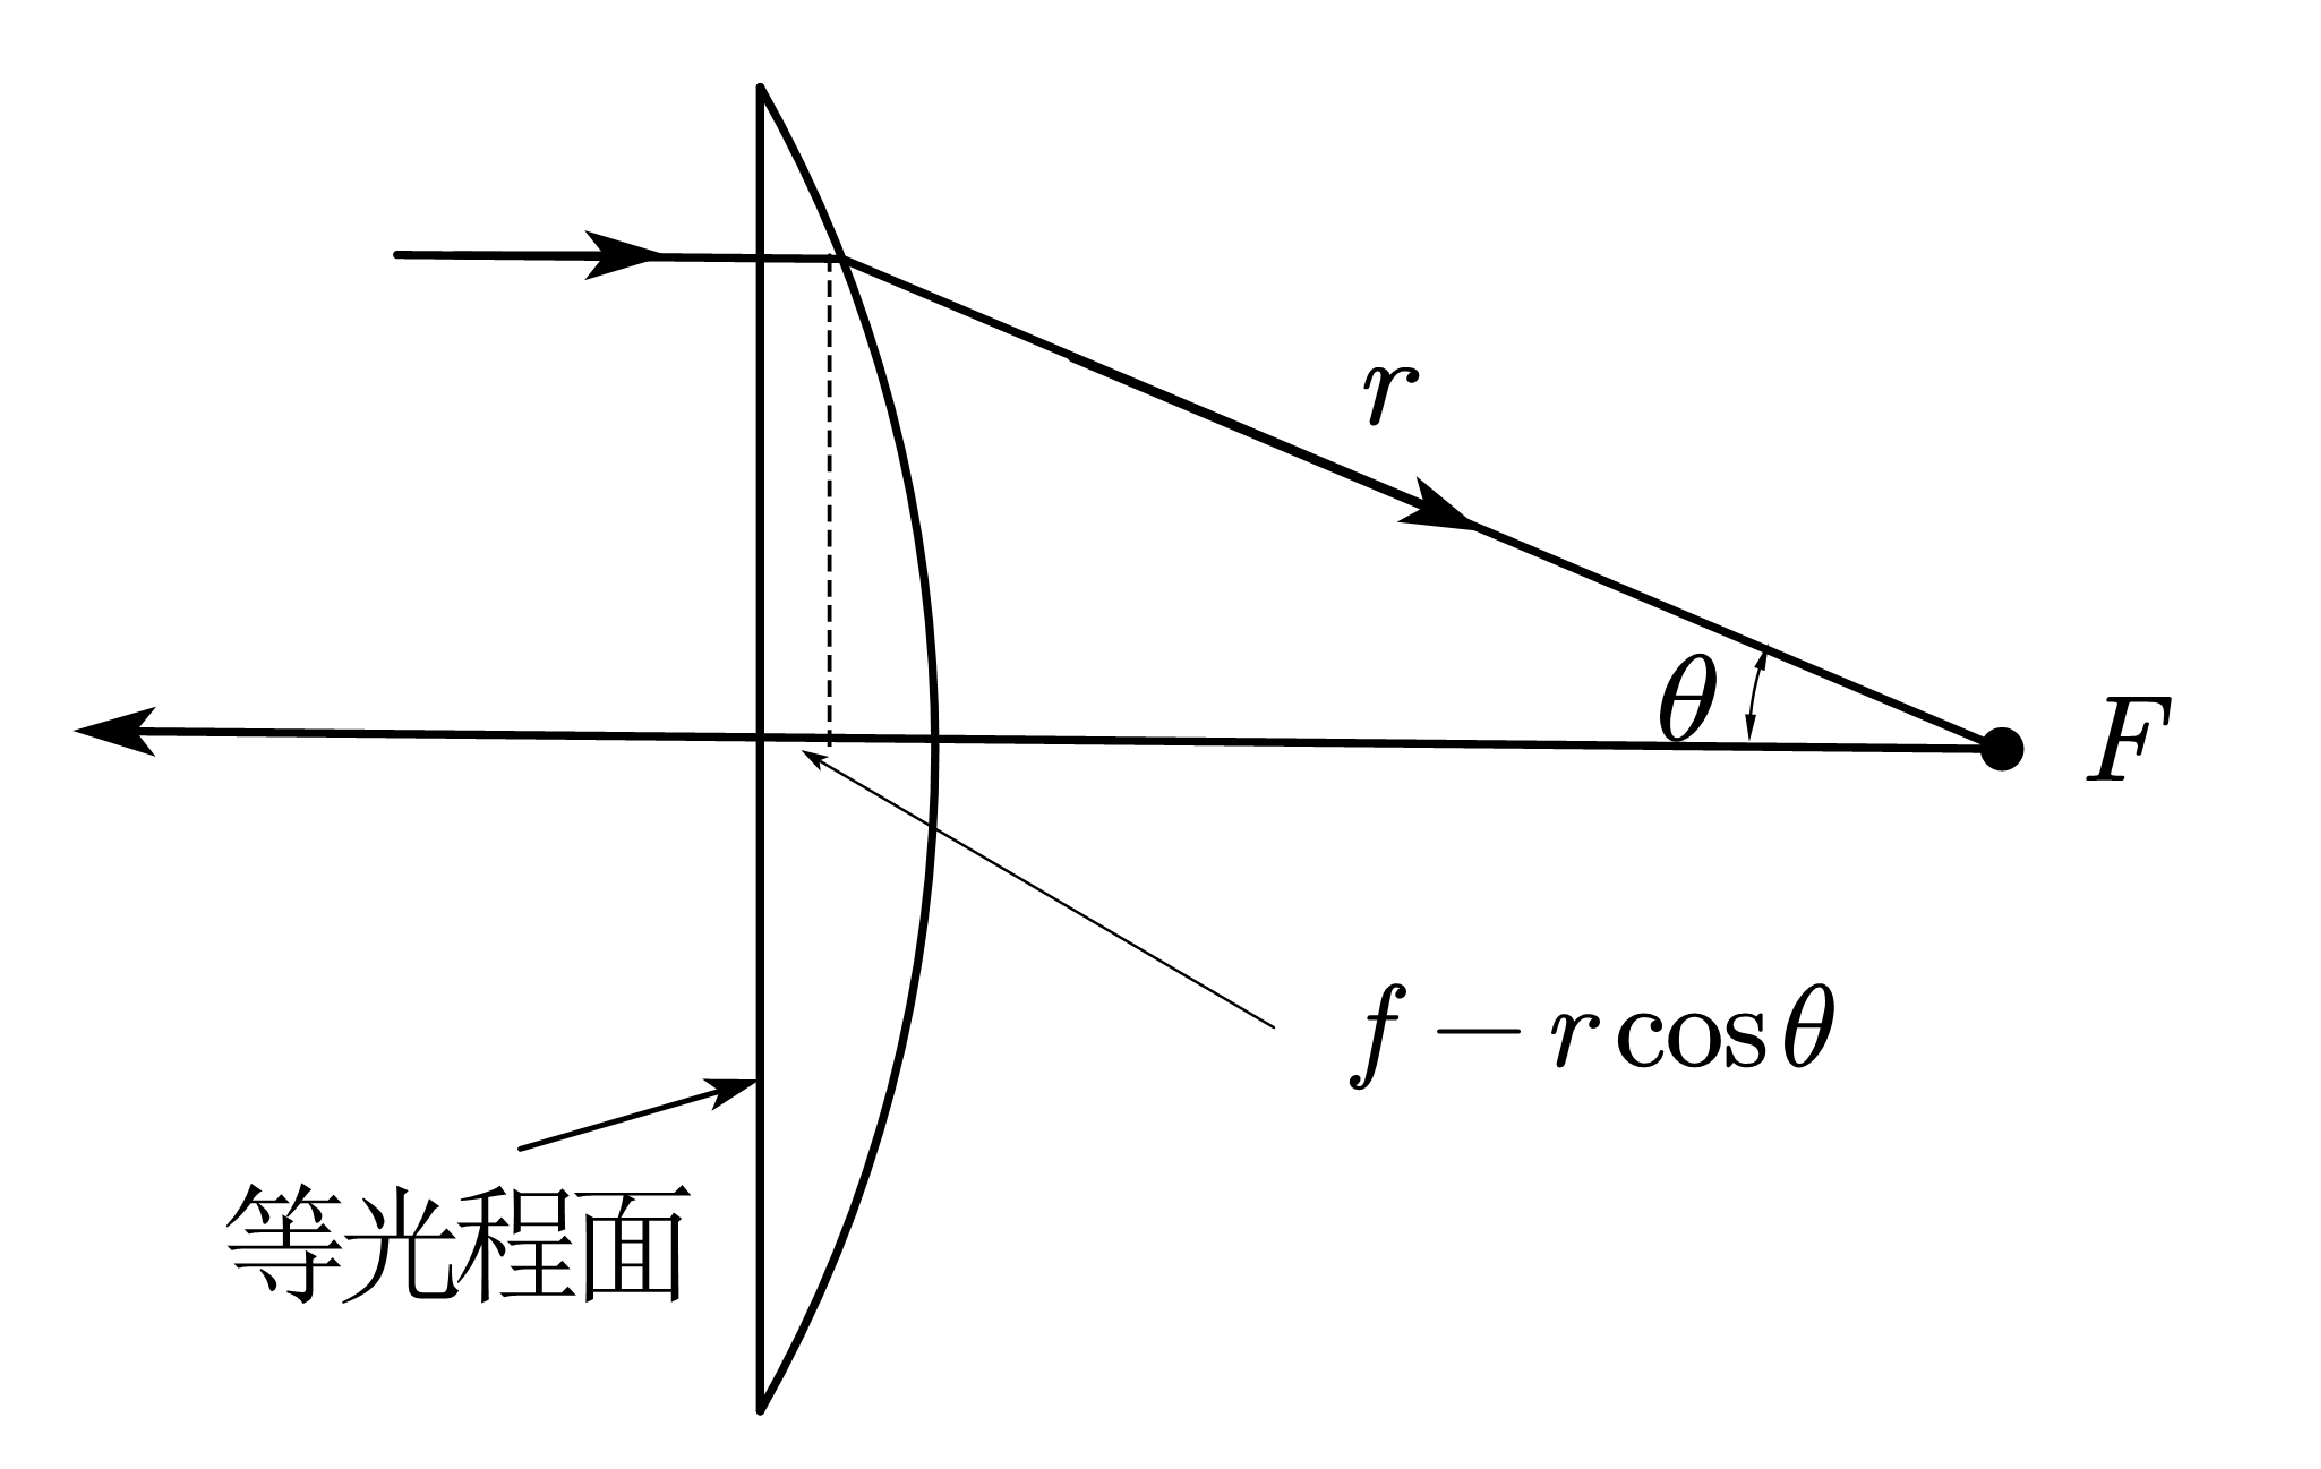
\includegraphics[width=0.7\linewidth]{../LatePic/TTJJX}
		\caption*{}
		\label{fig:ttjjx}
	\end{figure}
	如图, 可以认为光从左侧无穷远处一点选择光路并汇聚到焦点F, 根据费马原理, 每一条光路都是等光程的, 左侧从无穷远到透镜左平面平行光走过的光程相等, 所以光从左侧平面到焦点的光程也是相等的.
	
	以透镜焦点为极点, 朝左侧水平线为极轴建立极坐标系, 任取右侧平面上一点考究经过该点的光路, 该光路的光程等于中间水平光路的光程:
	\begin{equation}
		r+n\left( f-r\cos\theta\right)=nD+f-D 
	\end{equation}
	解得:
	$$
	r=\dfrac{\left( n-1\right) \left( D-f\right) }{1-n\cos\theta}
	$$
	这是圆锥曲线的极坐标方程, 因为 $n>1$, 所以右侧曲线是一个以 $n$ 为离心率的双曲线的一支.
	
	\nonumbersubsection{(2)}
	根据题意:
	\begin{equation}
		n(h)-1=\mu \dfrac{\rho}{m_0} \mathrm{e}^{-\tfrac{m_0gh}{k_BT}}
	\end{equation}
	据此可以求出环绕星球一圈的光路的光程:
	\begin{equation}
		S(h)=2\pi\left(R+h \right) n(h)=2\pi\left(R+h \right)\left( 1+\dfrac{\mu\rho}{m_0}\mathrm{e}^{-\tfrac{m_0gh}{k_BT}}\right) 
	\end{equation}
	对 $S(h)$ 求一次 $h$ 的导数:
	\begin{equation}
		S'(h)=2\pi\mathrm{e}^{-\tfrac{m_0gh}{k_BT}}\left( \mathrm{e}^{\tfrac{m_0gh}{k_BT}}+\dfrac{\mu\rho}{m_0}\left(\dfrac{1}{m_0}-\dfrac{g\left(R+h \right) }{k_BT} \right) \right) 
	\end{equation} 
	由于 $R\gg h$, 所以上式近似有:
	\begin{equation}
		S'(h)\approx2\pi\mathrm{e}^{-\tfrac{m_0gh}{k_BT}}\left( \mathrm{e}^{\tfrac{m_0gh}{k_BT}}+\dfrac{\mu\rho}{m_0}\left(\dfrac{1}{m_0}-\dfrac{gR}{k_BT} \right) \right) 
	\end{equation}
	解得:
	\begin{equation}
		h=\dfrac{k_BT}{m_0g}\ln \dfrac{\mu\rho}{m_0}\left(\dfrac{gR}{k_BT} -\dfrac{1}{m_0}\right) 
	\end{equation}
	\section{第六题}
	\nonumbersubsection{(1)}
	\nonumbersubsubsection{(i)}
	设两点电荷相距为 $r$
	\begin{equation}
		q_1U_{1}^{\prime}+q_2U_{2}^{\prime}=k\frac{q_1q_{2}^{\prime}}{r}+k\frac{q_2q_{1}^{\prime}}{r}
	\end{equation}
	\begin{equation}
		q_{1}^{\prime}U_1+q_{2}^{\prime}U_1=k\frac{q_{1}^{\prime}q_2}{r}+k\frac{q_{2}^{\prime}q_1}{r}
	\end{equation}
	注意到两方程的等号右边完全相同, 所以原命题得证.
	\nonumbersubsubsection{(ii)}
	假设当 $n=m\geqslant2$ 时命题成立, 即
	\begin{equation}
		\sum_{i=1}^m{q_iU_{i}^{\prime}=\sum_{i=1}^m{q_{i}^{\prime}U_i}}
	\end{equation}
	则当 $n=m+1$ 时有
	\begin{align}
		\sum_{i=1}^{m+1}{q_i}U_{i}^{\prime}&=q_1(U_{1}^{\prime}+k\frac{q_{m+1}^{\prime}}{r_{1,m+1}})+\cdots +q_m(U_{m}^{\prime}+k\frac{q_{m+1}^{\prime}}{r_{m,m+1}})\nonumber
		\\
		&\hphantom{=}+q_{m+1}\left( k\frac{q_{1}^{\prime}}{r_{1,m+1}}+\cdots +k\frac{q_{m}^{\prime}}{r_{m,m+1}} \right) \nonumber
		\\
		&=\sum_{i=1}^mq_iU_{i}^{\prime}+\sum_{i=1}^{m}k\dfrac{q_iq_{m+1}^{\prime}+q_i^{\prime}q_{m+1}}{r_{i,m+1}}
	\end{align}
	\begin{align}
		\sum_{i=1}^{m+1}{q_i}^{\prime}U_{i}&=q_1^{\prime}(U_{1}+k\frac{q_{m+1} }{r_{1,m+1}})+\cdots +q_m^{\prime}(U_{m}+k\frac{q_{m+1} }{r_{m,m+1}})\nonumber
		\\
		&\hphantom{=}+q_{m+1}^{\prime}\left( k\frac{q_{1}}{r_{1,m+1}}+\cdots +k\frac{q_{m} }{r_{m,m+1}} \right) \nonumber
		\\
		&=\sum_{i=1}^mq_i^\prime U_{i}+\sum_{i=1}^{m}k\dfrac{q_iq_{m+1}^{\prime}+q_i^{\prime}q_{m+1}}{r_{i,m+1}}
	\end{align}
	所以当 $n=m+1$ 时命题依旧成立, 根据归纳原理, 对于任意大于 2 的正整数 $n$, 此命题都成立.
	\nonumbersubsubsection{(iii)}
	根据已经证明的定理
	\begin{equation}
		\sum_{i=1}^n{q_iU_{i}^{\prime}=\sum_{i=1}^n{q_{i}^{\prime}U_i}}
	\end{equation}
	由于电容器是导体, 所以给定电荷后电容器是个等势体, 因此
	\begin{equation}
		U_i=U\qquad U_i^\prime=U^\prime
	\end{equation}
	是恒成立的,因此
	$$
	\dfrac{\displaystyle\sum_{i=1}^{n}q_i}{U}=\dfrac{\displaystyle\sum_{i=1}^{n}q_i^\prime}{U^\prime}
	$$
	因此
	$$
	C=C^\prime
	$$
	说明电容器的值与给定的电荷是无关的.
	\nonumbersubsection{(2)}
	\nonumbersubsubsection{(i)}
	\begin{figure}[H]
		\centering
		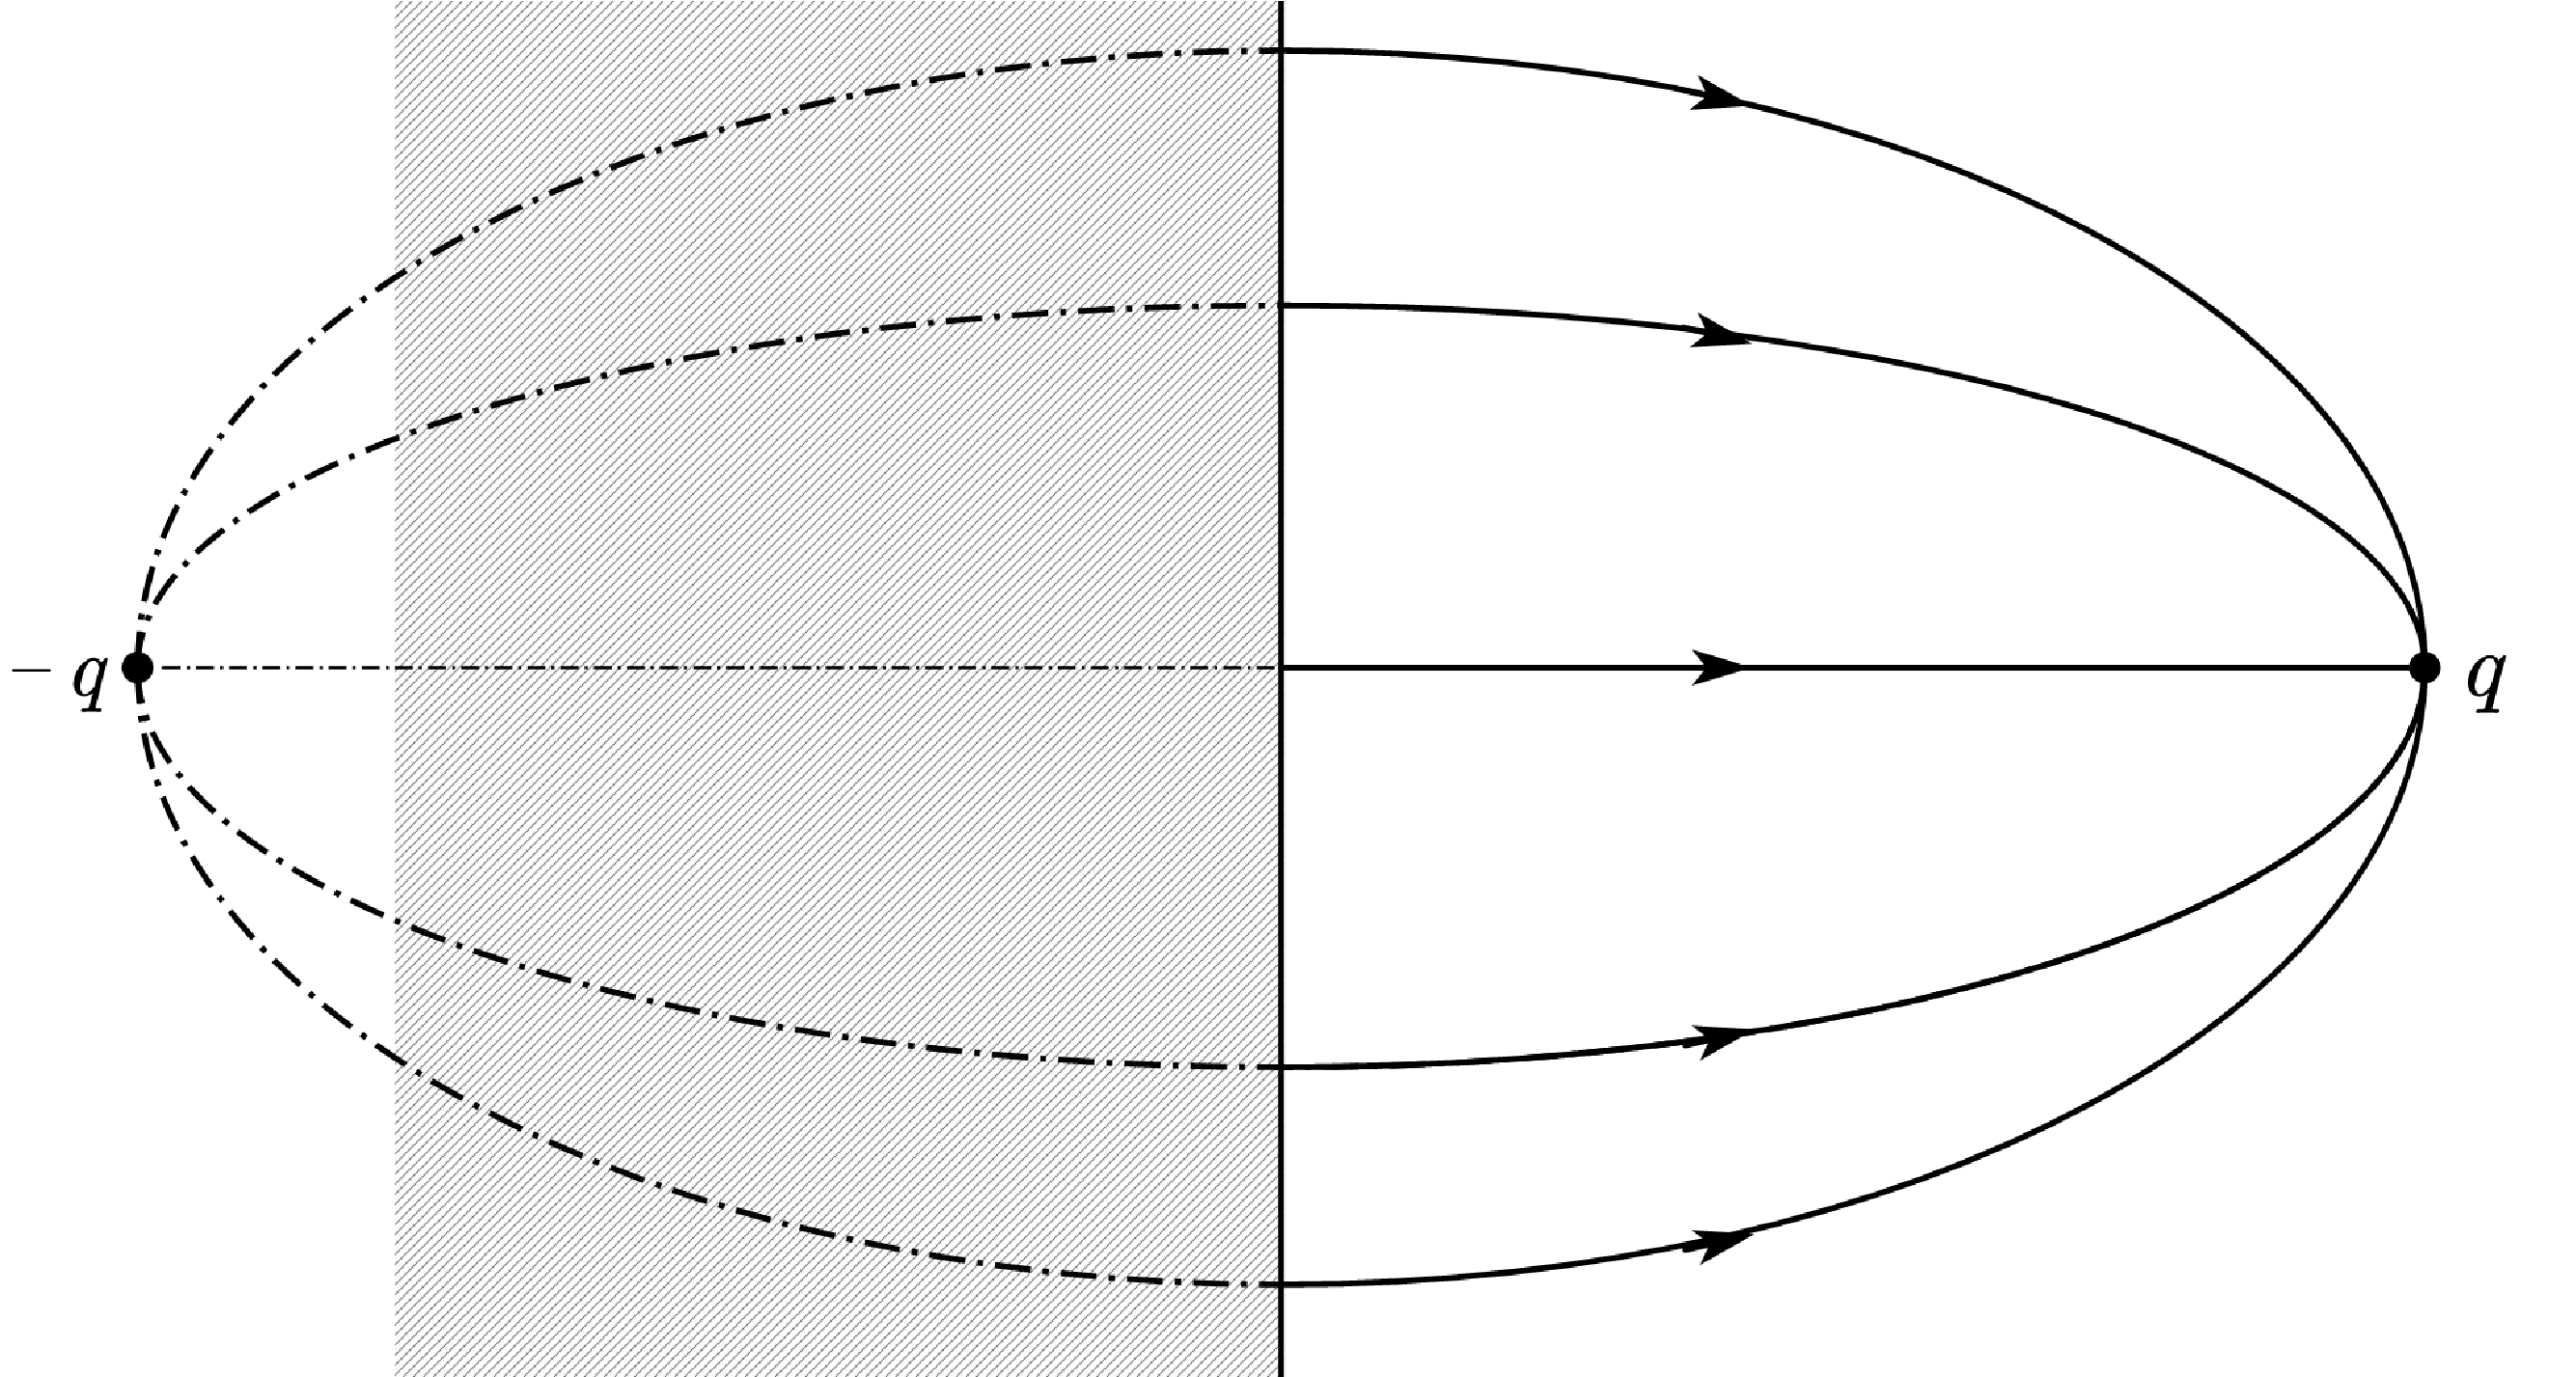
\includegraphics[width=0.9\linewidth]{../LatePic/PMDDH}
		\caption*{}
		\label{fig:pmddh}
	\end{figure}
	如图设像电荷带电量为 $-q$, 离板的距离为 $d$, 那么像电荷与点电荷在板上产生的电场处处垂直于板, 使得板成为等势体, 这和感应电荷与点电荷产生的电场使得板成为等势体效果一致, 根据题干提供的定理, 用像电荷产生的电场等效感应电荷产生的电场.
	
	考察点电荷的受力, 由库仑定律
	$$
		F=k\dfrac{q^2}{4d^2}
	$$
	方向垂直指向板面.
	\nonumbersubsubsection{(ii)}
	\begin{figure}[H]
		\centering
		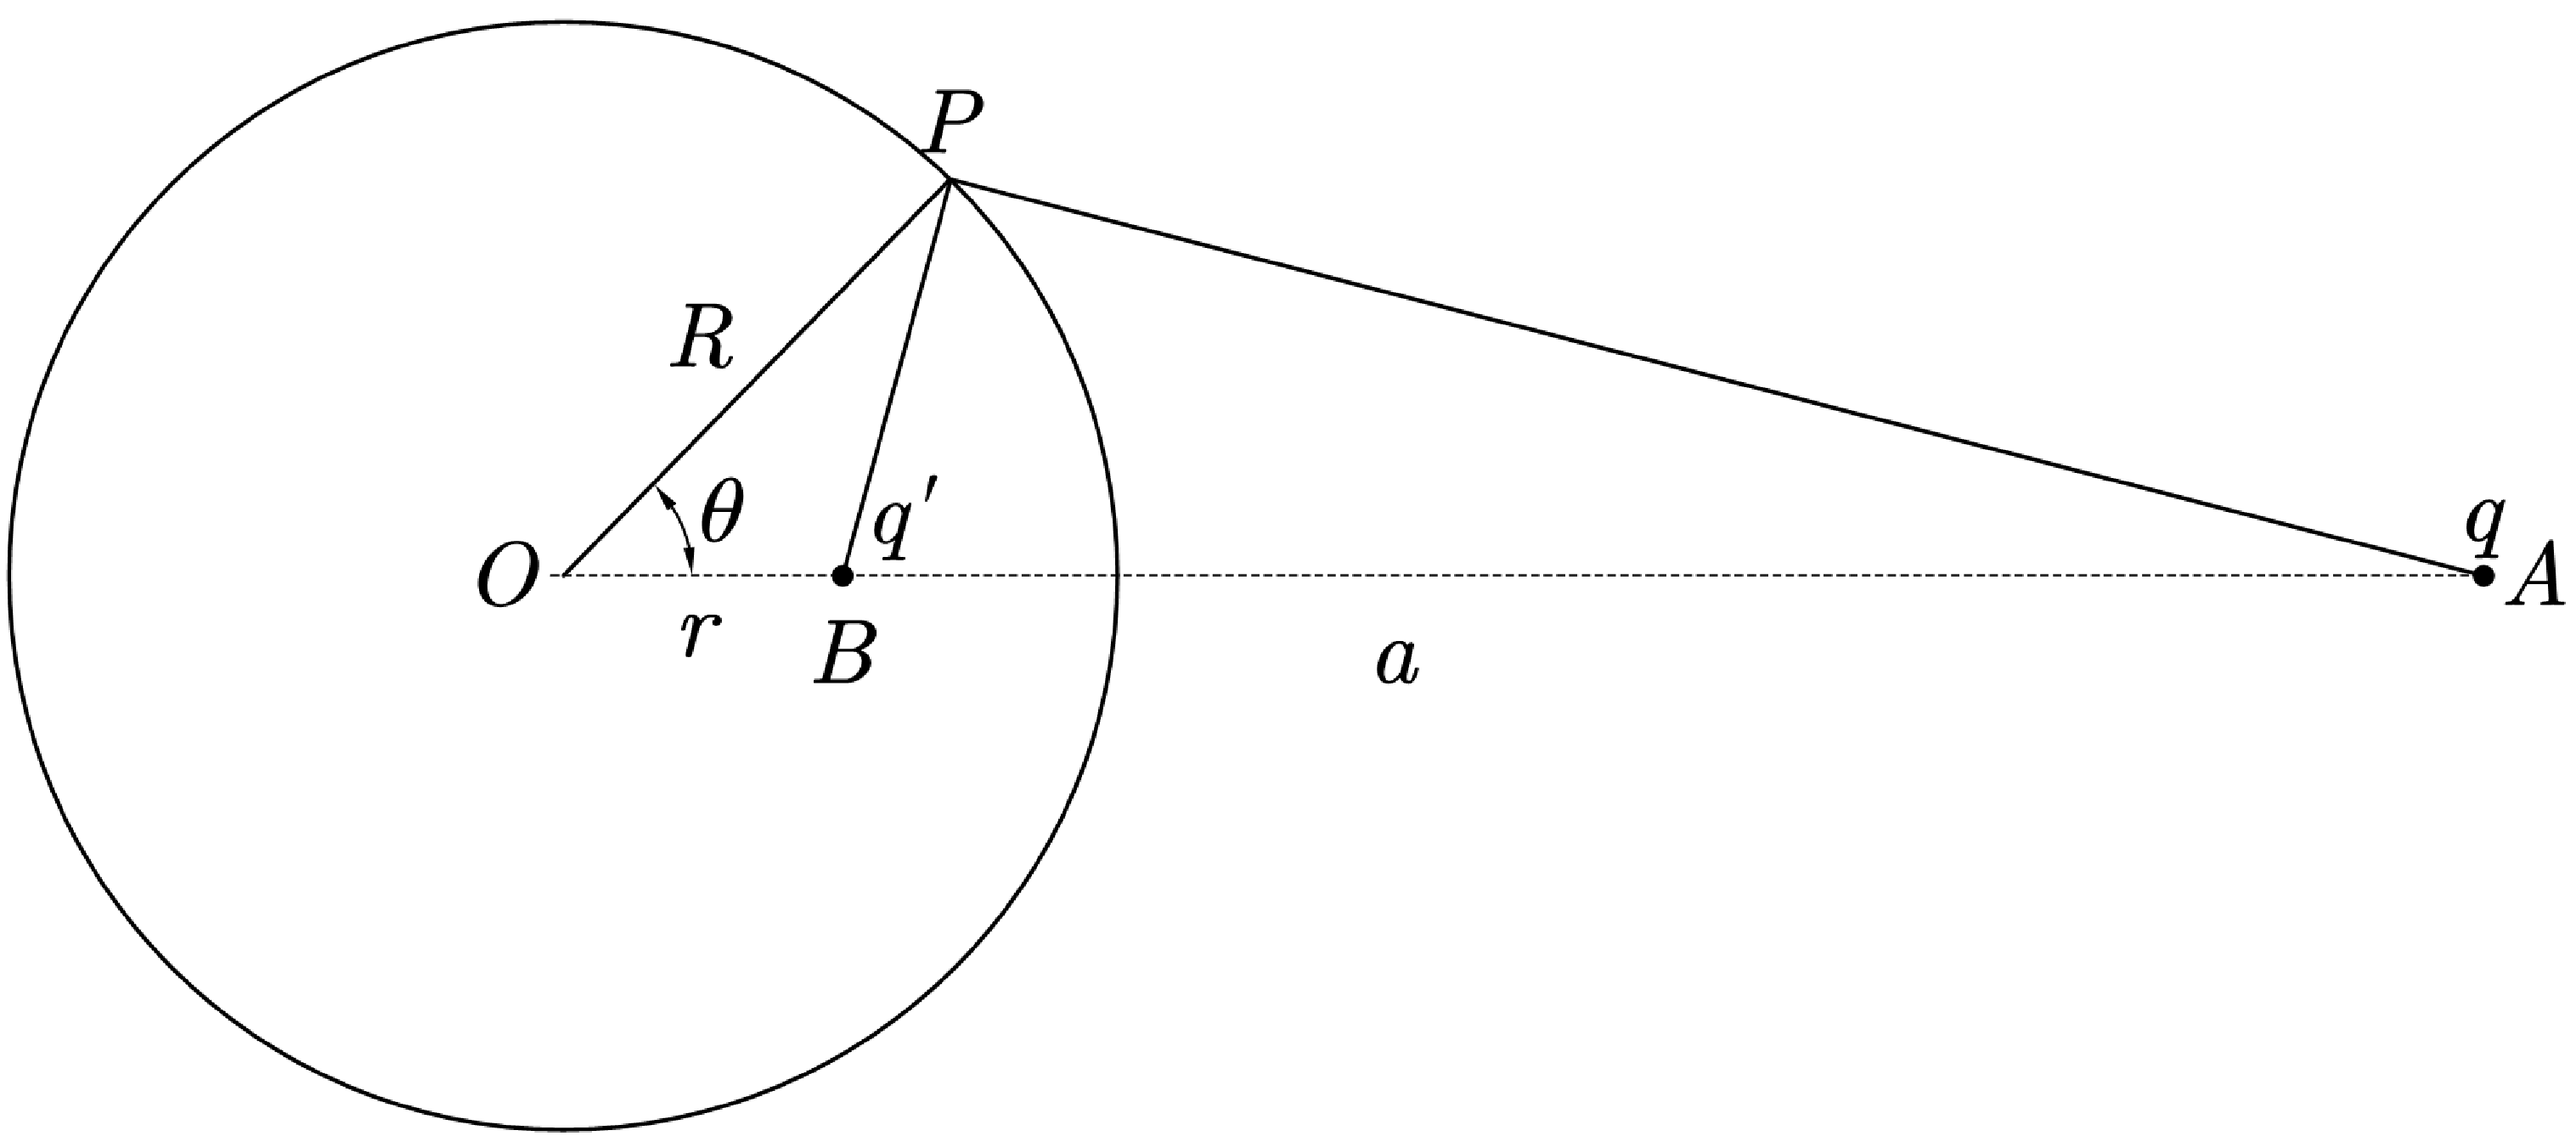
\includegraphics[width=0.9\linewidth]{../LatePic/QXJXDH}
		\caption*{}
		\label{fig:qxjxdh}
	\end{figure}
	如图, 在导体球上任找一点 $P$, 在 $AO$ 上找一点 $B$ 使得 $\bigtriangleup BPO\sim \bigtriangleup APO$, 并设 $\overline{OB}=r$, 这样就有
	\begin{equation}
		\dfrac{r}{R}=\dfrac{R}{a}
	\end{equation}
	解得
	$$
	r=\dfrac{R^2}{a}
	$$
	在 $B$ 点放置一像电荷 $q'$, 由于 $P$ 点是任找的, 只要像电荷的大小能使得 $P$ 点电势为 0 即可. 设 $\angle AOP=\theta$, 根据余弦定理
	\begin{align}
		U_P&=k\dfrac{q'}{\sqrt{R^2+r^2+2Rr\cos\theta}}+k\dfrac{q}{\sqrt{R^2+a^2+2Ra\cos\theta}}\nonumber
		\\
		&=k\dfrac{q'}{\sqrt{R^2+R^4/a^2+2R^3/a\cos\theta}}+k\dfrac{q}{\sqrt{R^2+a^2+2\cos\theta}}\nonumber
		\\
		&=k\dfrac{q'a/R}{\sqrt{R^2+a^2+2Ra\cos\theta}}+k\dfrac{q}{\sqrt{R^2+a^2+2Ra\cos\theta}}
	\end{align}
	所以 $q'=-\dfrac{R}{a}q$, 用像电荷的电场代替感应电荷的电场, 考虑点电荷的受力, 由库仑定律
	$$
	F=k\dfrac{aRq^2}{\left( a^2-R^2\right) }
	$$
	方向指向球心.
	\nonumbersubsection{(3)}
	考虑给定连接体电势 $U_0$, 再据此求出连接体的带电量, 为求出总的带电量, 考虑用像电荷代替净电荷, 其中像电荷的分布满足连接体是等势的.
	\begin{figure}[H]
		\centering
		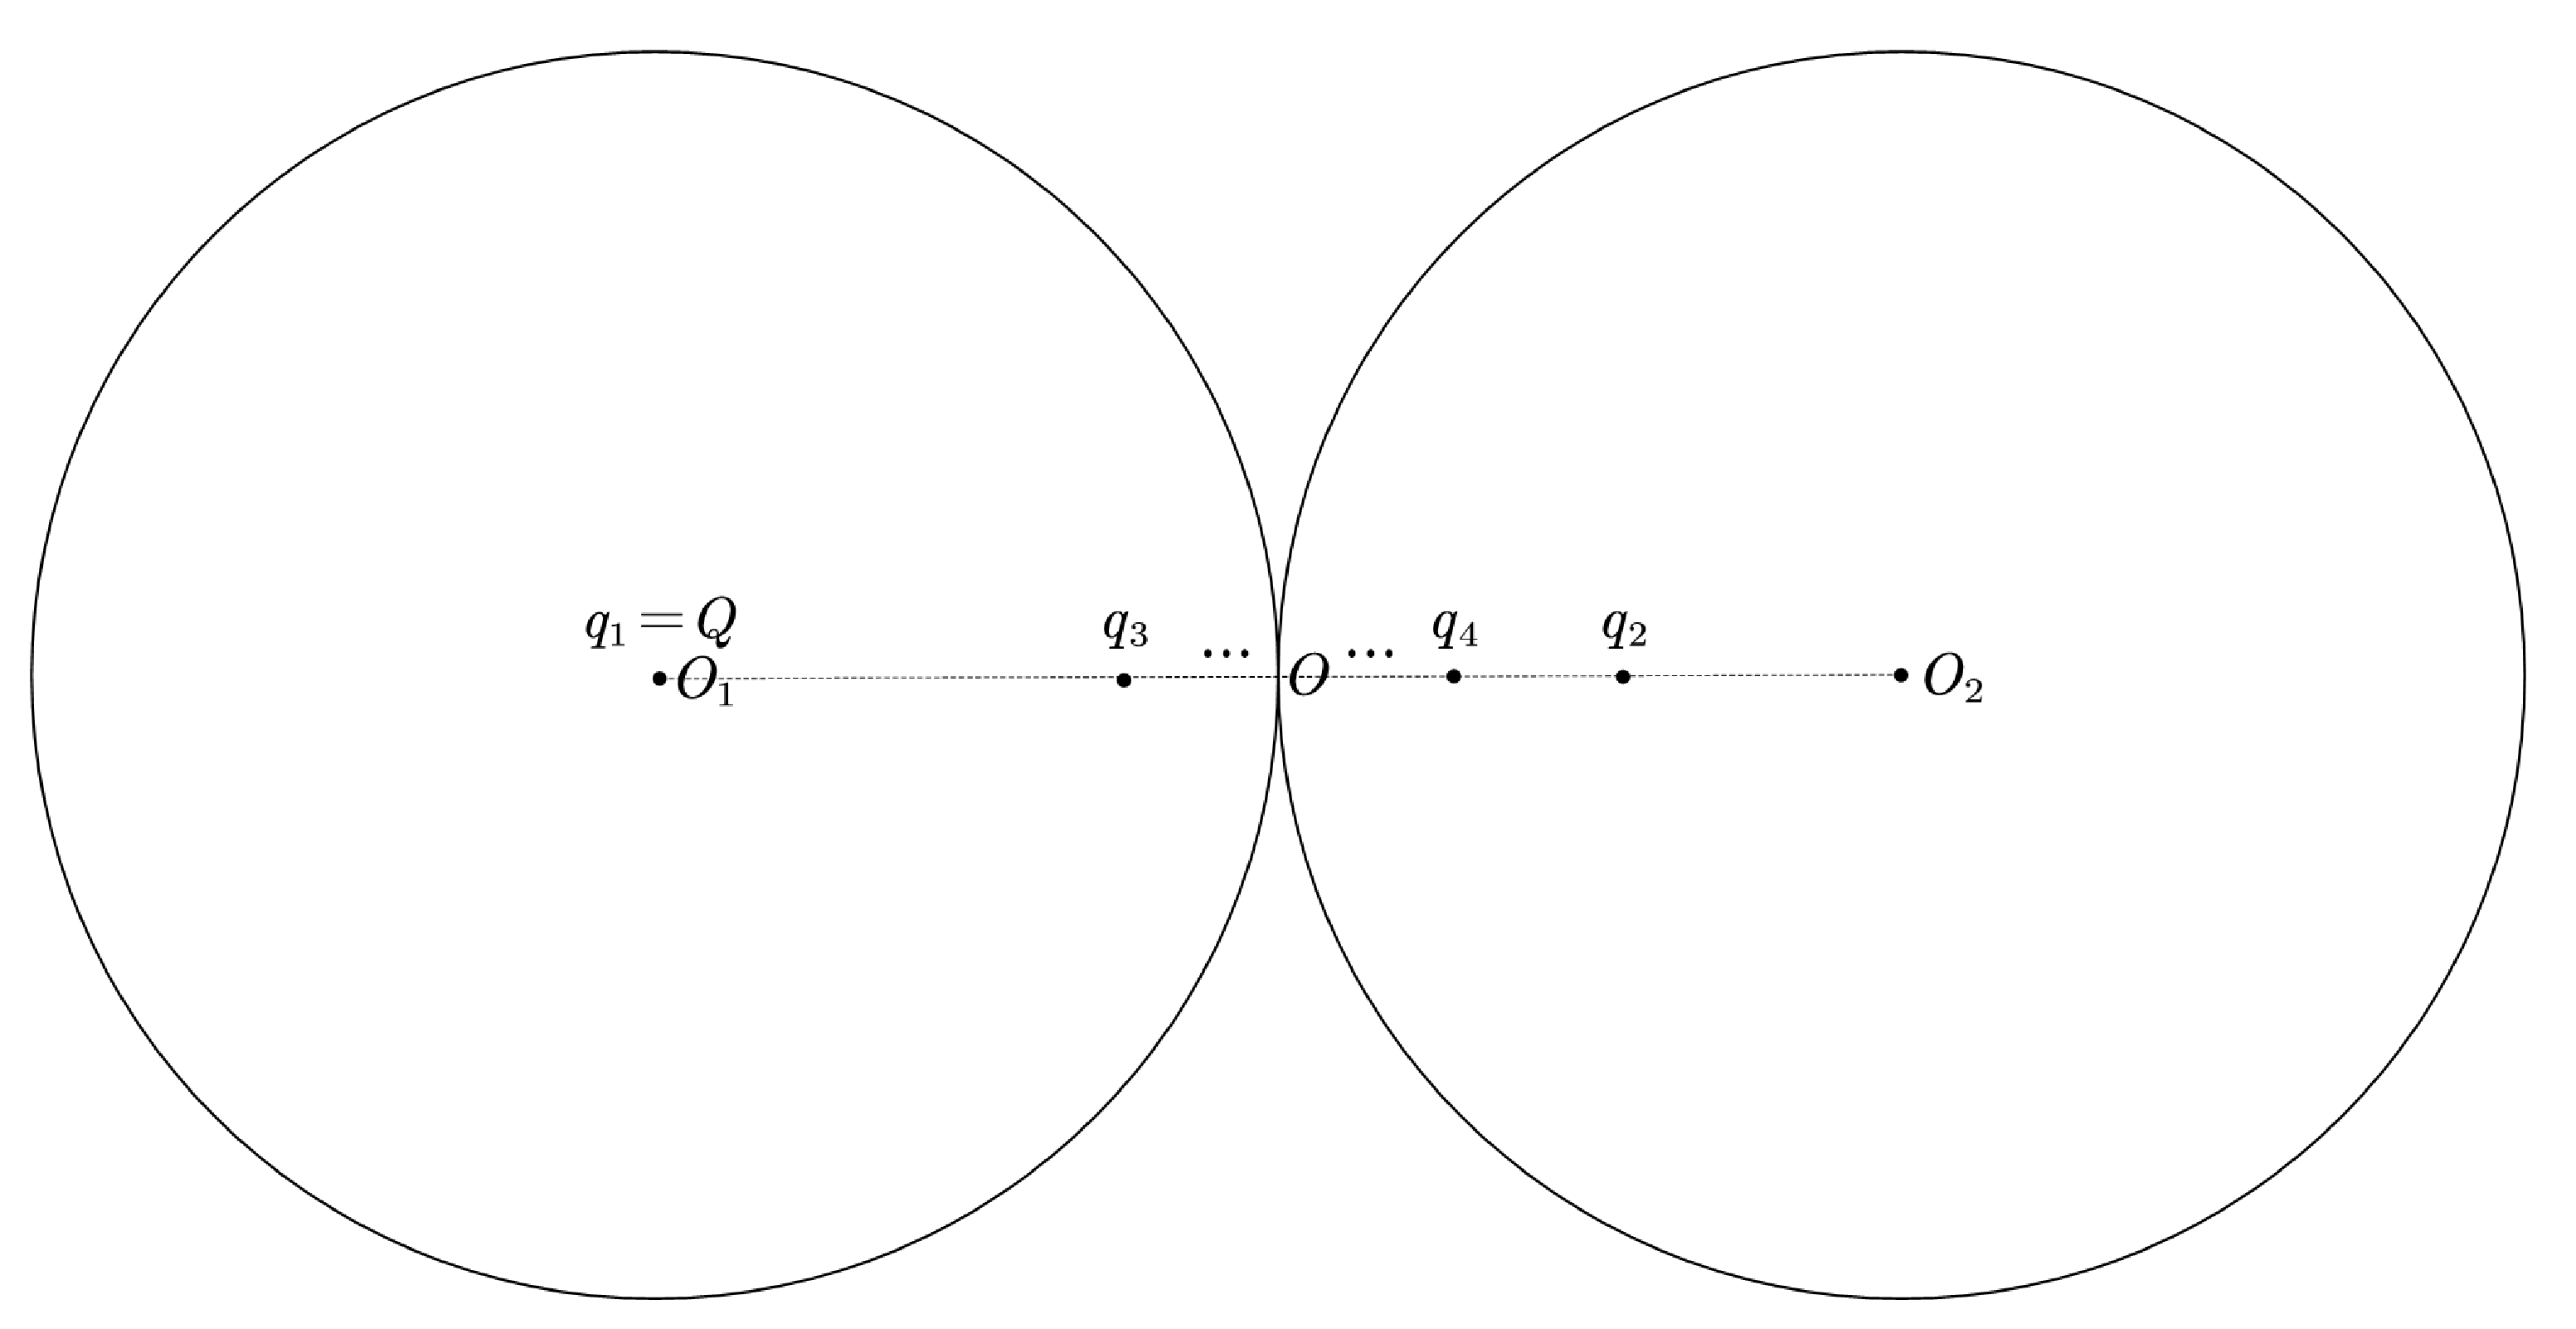
\includegraphics[width=0.9\linewidth]{../LatePic/WJJSDH}
		\caption*{}
		\label{fig:wjjsdh}
	\end{figure}
	
	如图所示, 设两球球心为 $O_1, O_2$, 设相切处为 $O$, 先考虑球 $O_1$, 当考虑球 $O_2$ 时只需要对称地进行如下构造, 此构造使得球 $O_1$ 的电势为 $U_0$, 球 $O_2$ 的电势为 0:
	
		为使得球 $O_1$ 的表面电势为 $U_0$, 设像电荷 $q_1=Q$ 在 $O_1$ 处, 其满足方程:
	\begin{equation}
		U_0=k\dfrac{Q}{R}
	\end{equation}
	但 $q_1$ 的存在使得球 $O_2$ 上产生了不等于 0 的附加电势, 为消除 $q_1$ 的影响设处于球 $O_2$ 内的像电荷 $q_2$, 但 $q_2$ 会在球 $O_1$ 上产生附加电荷, 于是在球 $O_1$ 内设像电荷 $q_3$ 来消除 $q_2$ 的影响……重复直至无穷.
	
	设第 $n$ 个像电荷距离所在球的球心距离为 $r_n$, 带电量为 $q_n$, 根据上一小题的结论
	\begin{equation}
		r_{n+1}=\dfrac{R^2}{2R-r_n}
	\end{equation}
	\begin{equation}
		q_{n+1}=\dfrac{R}{2R-r_n}q_n
	\end{equation}
	其中 $r_1=0, q_1=Q$, 解数列递推可得
	\begin{equation}
		r_n=\left(1-\dfrac{1}{n} \right)R 
	\end{equation}
	\begin{equation}
		q_n=\dfrac{(-1)^{n-1}}{n}Q
	\end{equation}
	所以连接体总的带电量为:
	\begin{equation}
		Q_{O_1O_2}=2\left( 1-\dfrac{1}{2}+\dfrac{1}{3}-\dfrac{1}{4}+\dfrac{1}{5}-\dfrac{1}{6}+\cdots\right)Q=2\ln2\dfrac{RU_0}{k}
	\end{equation}
	根据电容的定义
	$$
	C=\dfrac{Q_{O_1O_2}}{U_0}=2\ln2\dfrac{R}{k}
	$$
	\section*{第七题}
	先证明一个引理: 如图所示, 若半径满足关系 $r_n^2-r_{n-1}^2=r_{n-1}^2-r_{n-2}^2$ 的三个同心圆同时又满足: 最内侧同心圆内 ($0\sim r_{n-2}$) 无磁场, 而其余区域 ($r_{n-2}\sim r_{n-1}$、$r_{n-1}\sim r_{n}$) 有等大反向的匀强磁场, 则当粒子从圆心延半径方向出射, 通过两次同心圆边界后, 速度方向延长线过圆心.
	\begin{figure}[H]
		\centering
		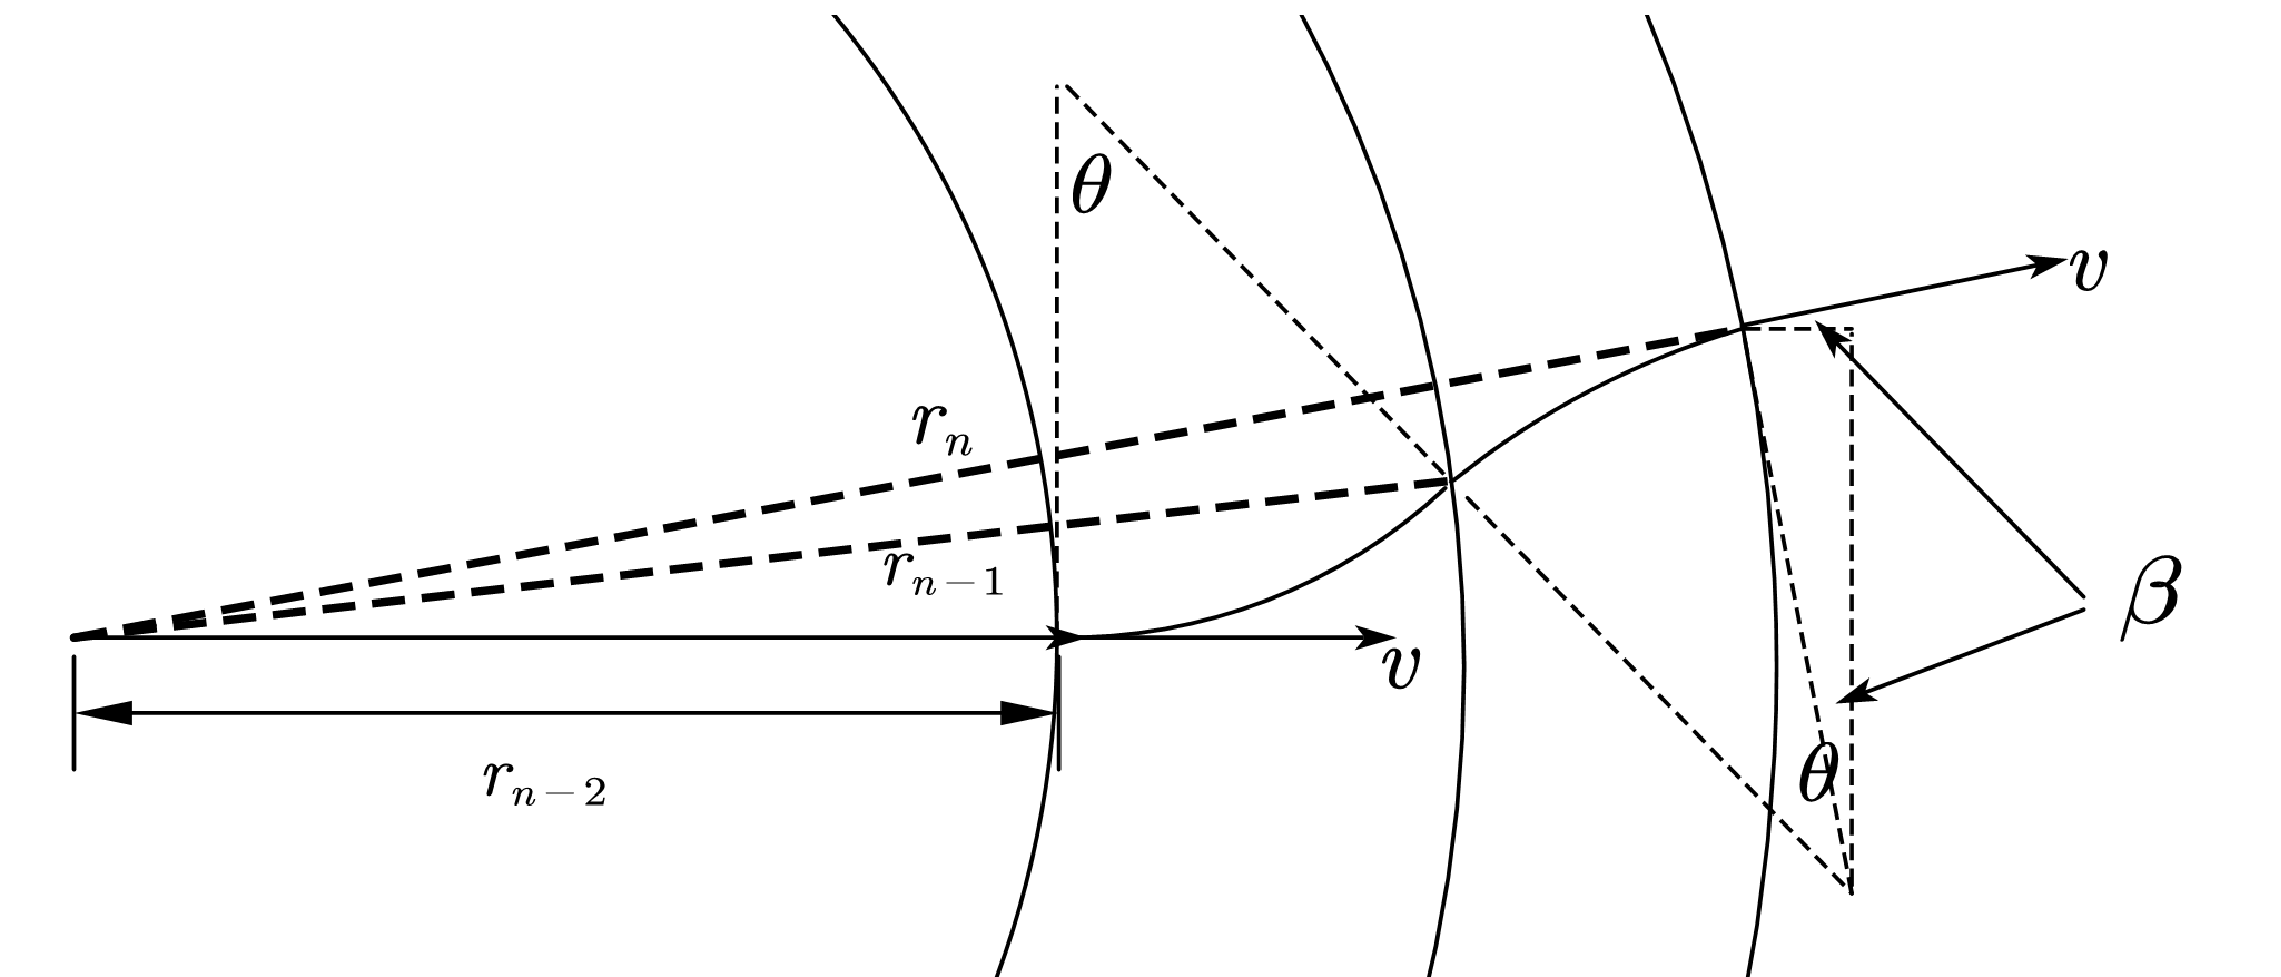
\includegraphics[width=0.9\linewidth]{../EarlyPic/Tiny_explain}
		\caption*{}
		\label{fig:tinyexplain}
	\end{figure}
	
	不妨令给定的长度 $r_1$ 为
	\begin{equation}
		r_n^2-r_{n-1}^2=r_{n-1}^2-r_{n-2}^2=r_1
	\end{equation}
	
	以粒子进入磁场的位置为参考点, 根据几何关系有
	\begin{align}
		\Delta x_1&=R\sin\theta
		\\
		\Delta y_1&=R\left( 1-\cos\theta\right)
		\\
		\Delta x_2&=R\left( \sin\theta-\sin\beta\right)  
		\\
		\Delta y_2&=R\left(\cos\beta-\cos\theta \right) 
	\end{align}
	
	说明一下符号的含义: 角标的阿拉伯数字表示是第几段磁场, $R$ 是粒子在磁场中的运动半径, $\theta$ 是粒子在第一段磁场中的偏转角, $\beta$ 是粒子在第二段磁场中的偏转角与 $\theta$ 的差.
	
	根据勾股定理:
	\begin{equation}
		\left( \Delta x_1+r_{n-2}\right)^2+\Delta y_1^2=r^2_{n-1} 
	\end{equation}
	\begin{equation}
		\left(  x_1+\Delta x_2+r_{n-2}\Delta\right)^2+\left( \Delta y_1+\Delta y_2\right)^2=r_n^2
	\end{equation}
	
	展开得到:
	\begin{equation}
		2\left(1-\cos\theta \right)R^2+2r_{n-2}\sin\theta R+r_1^2=0
	\end{equation}
	\begin{equation}
		\		\left( 3-2\cos\theta+\cos\beta-2\sin\theta\sin\beta-2\cos\theta\cos\beta\right)R^2+r_{n-2}\left(2\sin\theta -\sin\beta \right)R+r_1^2=0 
	\end{equation}
	
	两式相减:
	\begin{equation}
		\left( 1+\cos \beta -2\sin \theta \sin \beta -2\cos \theta \cos \beta \right) R^2-r_{n-2}\sin \beta R=0
	\end{equation}
	
	舍去 $R=0$ 这个不合理的解, 就得到了
	\begin{equation}
		R=\frac{r_{n-2}\sin \beta}{1+\cos \beta -2\sin \theta \sin \beta -2\cos \theta \cos \beta}
	\end{equation}
	
	设 $\alpha$ 为粒子离开第二段磁场时相对圆心的位移偏转角, 则要验证:
	\begin{equation}
		\tan\alpha=\tan\beta
	\end{equation}
	
	进行如下操作:
	
	\begin{align}
		 &\tan \alpha -\tan \beta =\frac{\Delta y_1+\Delta y_2}{\Delta x_1+\Delta x_2}-\frac{\sin \beta}{\sin \alpha} 
		 =\frac{R\left( 1-2\cos \theta +\cos \beta \right)}{R\left( 2\sin \theta -\sin \beta \right) +r_{n-2}}-\frac{\sin \alpha}{\cos \alpha}\nonumber\vspace{1em}
		 \\\nonumber
		 \\
		 &=\frac{R\left( 1+\cos \beta -2\sin \theta \sin \beta -2\cos \theta \cos \beta \right) -r_{n-2}\sin \beta}{\left( R\left( 2\sin \theta -\sin \beta \right) +r_{n-2} \right) \cos \theta}\nonumber
		 \\\nonumber
		 \\
		 &=\dfrac{\dfrac{r_{n-2}\sin \beta}{1+\cos \beta -2\sin \theta \sin \beta -2\cos \theta \cos \beta}\left( 1+\cos \beta -2\sin \theta \sin \beta -2\cos \theta \cos \beta \right) -r_{n-2}\sin \beta}{\left( R\left( 2\sin \theta -\sin \beta \right) +r_{n-2} \right) \cos \theta}\nonumber
		 \\\nonumber
		 \\
		 &=\dfrac{r_{n-2}\sin\beta-r_{n-2}\sin\beta}{\left( R\left( 2\sin \theta -\sin \beta \right) +r_{n-2} \right) \cos \theta}=0
	\end{align}
	
	所以 $\alpha=\beta$, 证明完毕.
	
	\nonumbersubsection{(1)}
	\nonumbersubsubsection{(i)}
	$v_\mathrm{min}=\dfrac{qBr}{2m}$

	
	\nonumbersubsubsection{(ii)}
	根据引理, 令 $r_{n-2}\rightarrow0$, 即可得证. 其他方法利用几何关系推演, 或者利用高级的结论如正则角动量(要推导, 否则适当扣分)言之有理可得分.
	
	\nonumbersubsection{(2)}
	\nonumbersubsubsection{(i)}
	利用引理, 当粒子穿过外面两层磁场时, 会沿半径方向垂直射入第三层磁场, 以此类推会回到(1)(ii)的情形. 其他方法言之有理可得分.

	\nonumbersubsubsection{(ii)}
	$v_\mathrm{min}=\dfrac{qBr}{2m}$
	
\end{document}